\documentclass[a4paper,hidelinks,12pt]{article}
% \usepackage{geometry}
\usepackage{amsmath,graphicx}
\usepackage[utf8]{inputenc}
\usepackage[russian]{babel}
\usepackage{indentfirst}
\usepackage{colortbl}
\usepackage{setspace}
\usepackage{float}
\usepackage[noend]{algorithmic}
\usepackage[nottoc,notlot,notlof]{tocbibind}
\usepackage{amssymb}
\usepackage{amsmath}
\usepackage{graphicx}
\usepackage{listings}
\usepackage{subcaption}
\usepackage[boxruled]{algorithm2e}
\usepackage{setspace}
\usepackage{natbib}
\usepackage{minted}
\usepackage{subcaption}
    
\SetKwInput{KwData}{Входные данные}
\SetKwInput{KwResult}{Результат}

\SetKwIF{If}{ElseIf}{Else}{если}{тогда}{иначе если}{иначе}{конец если}
\SetKwFor{For}{для}{сделать}{конец для}

\SetKw{Return}{вернуть}
\SetKw{End}{конец}
\SetKw{KwIn}{в}

\usepackage{xcolor}
\definecolor{gray}{rgb}{0.4,0.4,0.4}
\definecolor{darkblue}{rgb}{0.0,0.0,0.6}
\definecolor{cyan}{rgb}{0.0,0.5,0.5}
\definecolor{maroon}{rgb}{0.5,0,0}
\definecolor{darkgreen}{rgb}{0,0.5,0}

\usepackage[left=3cm,right=2cm,top=2cm,bottom=2cm,bindingoffset=0cm]{geometry}
\setcounter{secnumdepth}{4}
% \linespread{1.6}
\setlength{\baselineskip}{1.6}
\usepackage{xcolor}
\usepackage{pdfcomment}

\newcommand{\todo}[1]{\textcolor{red}{\texttt{#1}}}

\usepackage{wrapfig}
\usepackage{graphicx}
\graphicspath{ {./pictures/} }

\everymath{\displaystyle}

% \tolerance=1
% \emergencystretch=\maxdimen
% \hyphenpenalty=10000
% \hbadness=10000

\begin {document}
\begin {titlepage}
\thispagestyle{empty}

\begin{center}
\vspace{-1cm}

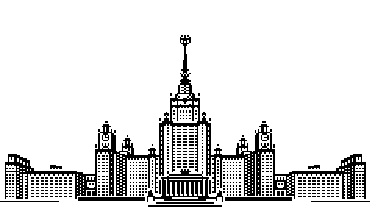
\includegraphics[width=0.5\textwidth]{msu}\\
Московский Государственный Университет им. М.В. Ломоносова\\
Факультет Вычислительной Математики и Кибернетики\\

\vspace{3cm}

{\Large Кожевников Евгений Владимирович}

\vspace{1cm}

% par made the trick here idk why
{\LARGE\bfseries Отчёт заданию №2 в рамках курса <<Суперкомпьютерное моделирование\\ и технологии>>\par}

\vspace{1cm}

{\Large\bfseries Вариант 8}

\end{center}

\vfill

\begin{center}
Москва, 2023
\end{center}

\end{titlepage}

\setcounter{page}{2}
\onehalfspacing

\newpage
\tableofcontents

\setlength{\parskip}{0.8em}
\newpage

\section{Постановка задачи}

Рассматривается дифференциальная задача для для трёхмерного гиперболического уравнения в области, представляющей из себя прямоугольный параллелепипед.

В трёхмерной замкнутой области
% 
\[ \Omega  = [0 \leqslant x \leqslant L_x] \times [0 \leqslant y \leqslant L_y] \times [0 \leqslant z \leqslant L_z] \]
% 
\noindent для \( 0 < t \leqslant T \) требуется найти решение \( u(x,y,z,t) \) уравнения в частных производных
% 
\[ \frac{\partial ^ 2 u}{\partial t ^ 2} = a ^ 2 \Delta u \]
% 
\noindent с начальными условиями
% 
\begin{align*}
u |_{t=0} &= \varphi (x, y, z) \\
\left.\frac{\partial u}{\partial t}\right|_{t=0} &= 0
\end{align*}
% 
\noindent при условии, что на границе области заданы периодические граничные условия
% 
\begin{align*}
    u(0, y, z, t) &= u(L_x, y, z, t) & u_x(0, y, z, t) &= u_x(L_x, y, z, t) \\
    u(x, 0, z, t) &= u(x, L_y, z, t) & u_y(x, 0, z, t) &= u_y(x, L_y, z, t) \\
    u(x, y, 0, t) &= u(x, y, L_z, t) & u_z(x, y, 0, t) &= u_y(x, y, L_z, t) \\
\end{align*}

В соответствии с \textbf{вариантом 8}, аналитическое решение задано следующим образом:
% 
\begin{align*}
    u_{analytical} &= \sin{\left( \frac{2\pi}{L_x} x \right)}
        \cdot \sin{\left( \frac{4\pi}{L_y}y \right)}
        \cdot \sin{\left( \frac{6\pi}{L_z} z \right)}
        \cdot \cos{\left( a_t \cdot t \right)} \\
    a_t &= \sqrt{\frac{4}{L_x^2} + \frac{16}{L_y^2} + \frac{36}{L_z^2}} \\
    a^2 &= 1
\end{align*}

\newpage

\section{Численный метод решения задачи}

Введём на \( \Omega \) сетку \( \omega_{h\tau} = \overline{\omega}_h \times \omega_\tau \). Через \( \omega_h \) обозначим множество внутренних, а через \( \gamma_h \) --- множество граничных узлов сетки \( \overline{\omega}_h \).

Через $\Delta_h$ обозначим семиточечный разностный аналог оператора Лапласа.

Для начала счёта определим значения \( u \) для первых двух итераций:
% 
\begin{align*}
    u^0_{ijk} &= \varphi (x_i, y_j, z_k) \in \overline{\omega_h} \\
    u^1_{ijk} &=
      \begin{cases}
      u^0_{ijk} + a^2\frac{\tau^2}{2}\Delta_h\varphi(x_i,y_j,z_k), & (x_i, y_j, z_k) \in \omega_h \\
      u_{analytical}(x_i, y_j, z_k, \tau), & (x_i, y_j, z_k) \in \gamma_h
    \end{cases}
\end{align*}

Из явной разностной схемы 

\[ \frac{u^{n+1}_{ijk} - 2u^n_{ijk} + u^{n-1}_{ijk}}{ \tau^2} = a^2 \Delta_h u^n,\quad (x_i, y_j, z_k) \in \omega_h \]

\noindent выразим значения $u^{n+1}_{ijk}$ на $(n+1)$-м шаге через значения на предыдущих слоях:

\[ u^{n+1}_{ijk} = 2u^n_{ijk} - u^{n-1}_{ijk} + \tau^2 a^2 \Delta_h u^n \]

\section{Программная реализация алгоритма с использованием технологий OpenMP}

Для распараллеливания алгоритма численного решения задачи была использована директива \texttt{\#pragma omp parallel for collapse(N)} для каждого гнезда циклов.

Для вывода отладочной информации с значениями аналитического и численного решения в узлах была использована однопоточная реализация. Это было сделано из-за незначительности времени вычислений по сравнению с временем записи значений на диск.

\newpage
\section{Результаты запусков на IBM Polus}

Для компиляции использовался стандартный компилятор GNU. Оптимизации были отключены, так как они рассчитаны в основном на однопоточные программы и ухудшают производительность программ, распараллеленных с помощью OpenMP.
% 
\begin{minted}[linenos=false]{bash}
g++ -std=c++11 -O0 -o v8 -fopenmp v8.cpp
\end{minted}

Для запуска использовался следующий командный файл для утилиты \texttt{bsub}:
% 
\begin{minted}[linenos=true]{bash}
#BSUB -n N
#BSUB -W 00:15
#BSUB -o "thread_M.out"
#BSUB -e "thread_M.err"
#BSUB -R "span[hosts=1]"
OMP_NUM_THREADS=M ./v8
\end{minted}
% 
\noindent где M  --- число OpenMP нитей, с которым запустится программа, а N --- число выделенных ядер процессора. M и N для всех запусков выбирались с соотношением $\frac{M}{N} = 2$.
% 
\begin{minted}[linenos=false]{bash}
bsub < script.lsf
\end{minted}

Ускорение $S$ и погрешность $\delta$ вычислялись следующим образом:
\begin{align*}
    S &= \frac{T|_{n threads}}{T|_{n threads = 1}} \\
    \delta &= \sum_{(x_i, y_j, z_k) \in \omega_h} \left| u_{analytical}(x_i, y_j, z_k, T) - u_{calculated}(x_i, y_j, z_k, T) \right|
\end{align*}

Рассматривалось $K=20$ эпох симуляции от $T=0$ до $T=0.001$. В итоговых таблицах представлено значение погрешности $\delta$ на заключительной эпохе симуляции.

\subsection{L = 1}

{
\centering
\noindent\begin{tabular}{|p{2cm}|p{2.5cm}|p{2.5cm}|p{2cm}|p{3cm}|}
    \hline
    \textit{Число OpenMP нитей} & \textit{Число точек сетки }$N^3$ & \textit{Время решения T (ms)} & \textit{Ускорение S} & \textit{Погрешность }$\delta$ \\
    \hline
    1 & $128^3$ & 14827.8 & 1 & 0.00209787 \\
    2 & $128^3$ & 6911.27 & 2.15 & 0.00209787 \\
    4 & $128^3$ & 5171.96 & 2.87 & 0.00209787 \\
    8 & $128^3$ & 3473.81 & 4.27 & 0.00209787 \\
    16 & $128^3$ & 3097.21 & 4.79 & 0.00209787 \\
    \hline
    1 & $256^3$ & 94378.8 & 1 & 0.00420157 \\
    4 & $256^3$ & 36181.3 & 2.61 & 0.00420157 \\
    8 & $256^3$ & 25097.1 & 3.76 & 0.00420157 \\
    16 & $256^3$ & 19657.7 & 4.80 & 0.00420157 \\
    32 & $256^3$ & 14909 & 6.33 & 0.00420157 \\
    \hline
\end{tabular}
}

\subsubsection{Графики для N=128}

\begin{figure}[H]
\begin{subfigure}{.33\textwidth}
  \centering
  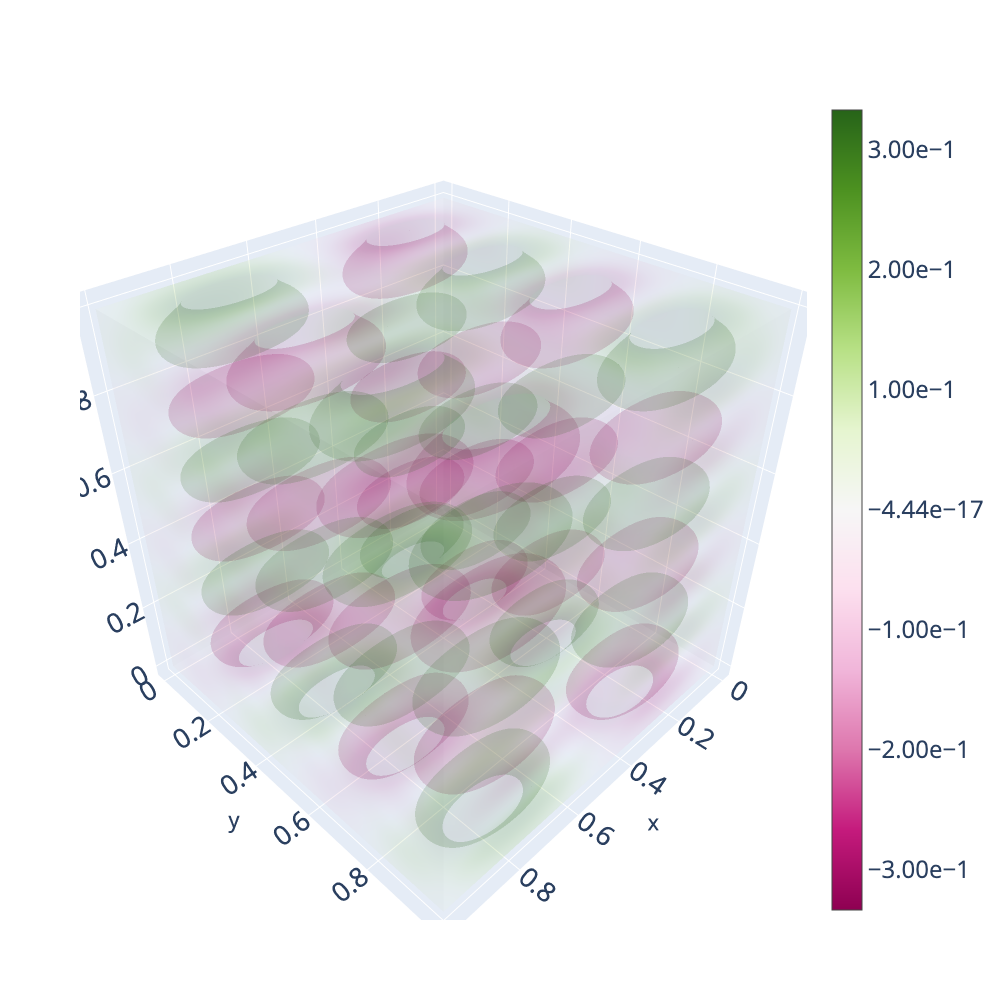
\includegraphics[width=\linewidth]{pictures/1_L1_128_analytical.png}
  \caption{$u_{analytical}$}
\end{subfigure}%
\begin{subfigure}{.33\textwidth}
  \centering
  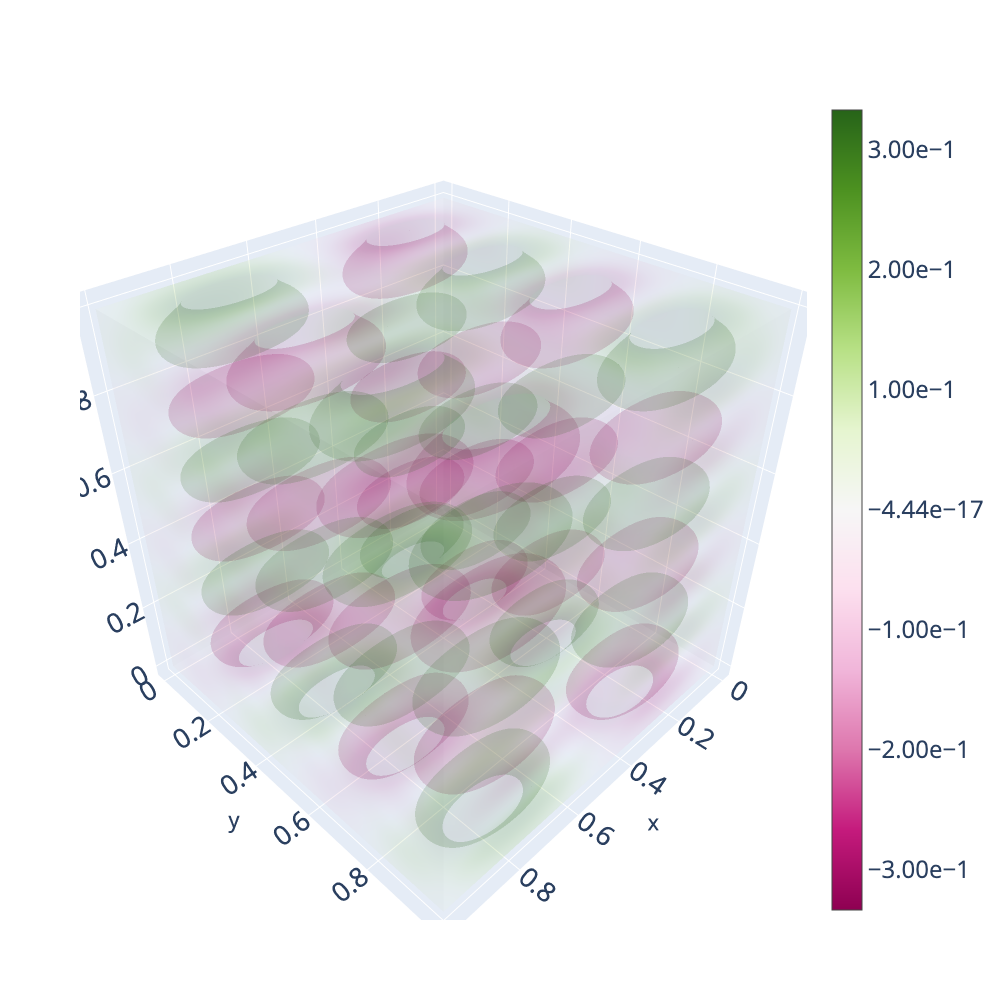
\includegraphics[width=\linewidth]{pictures/1_L1_128_calculated.png}
  \caption{$u_{calculated}$}
\end{subfigure}%
\begin{subfigure}{.33\textwidth}
  \centering
  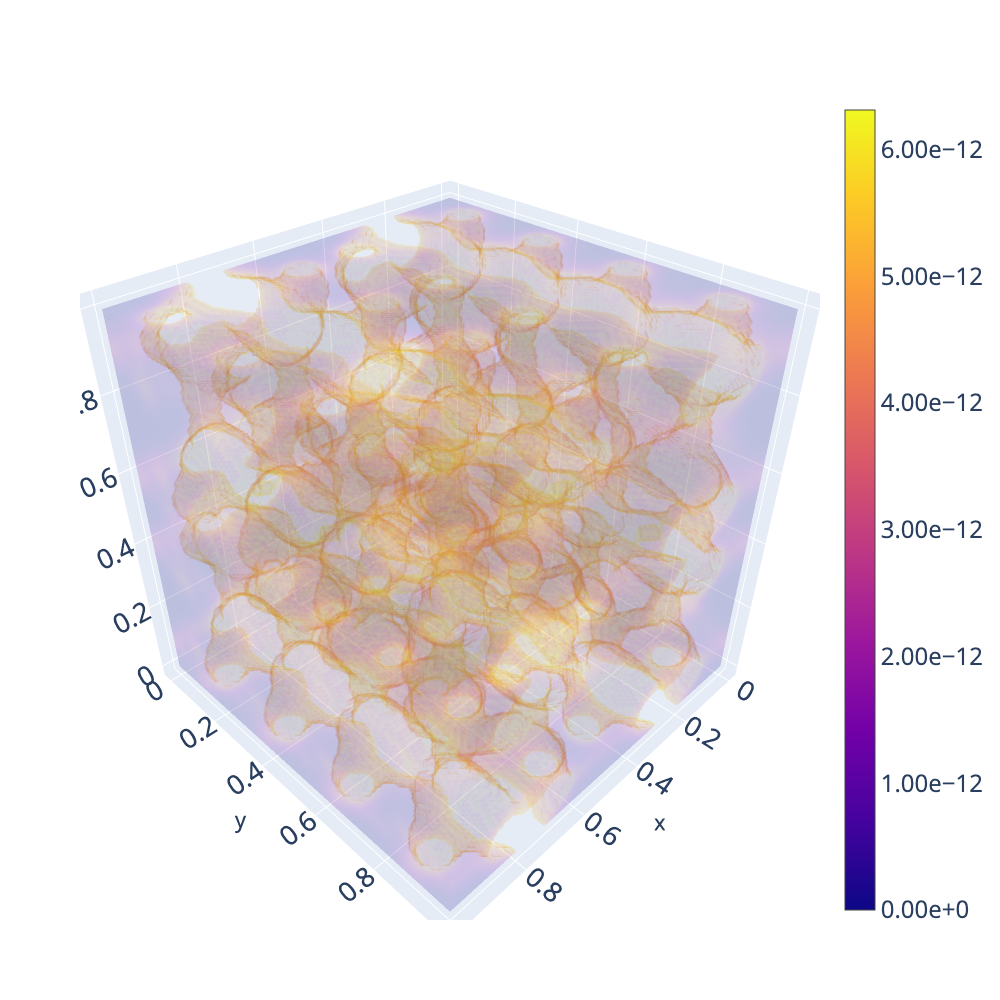
\includegraphics[width=\linewidth]{pictures/1_L1_128_diff.png}
  \caption{погрешность}
\end{subfigure}%
\caption{1 эпоха}
\label{fig:fig}
\end{figure}

\begin{figure}[H]
\begin{subfigure}{.33\textwidth}
  \centering
  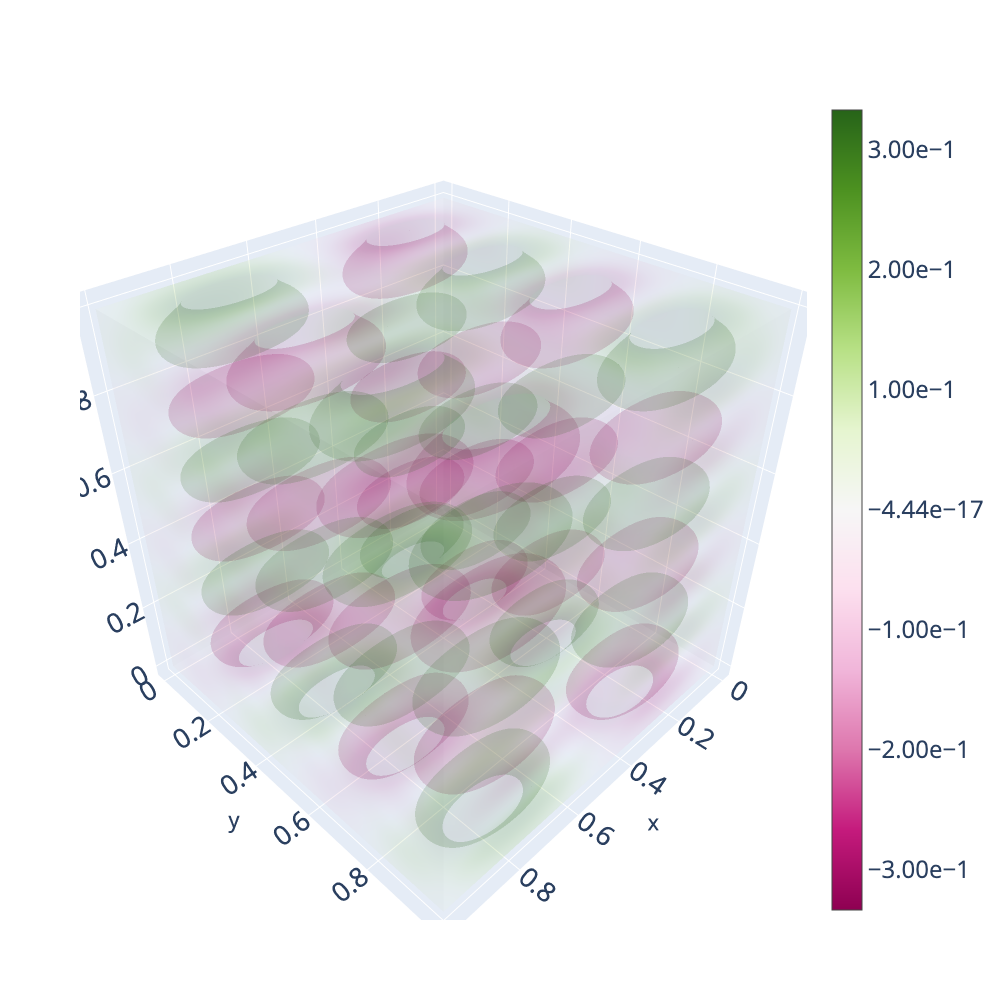
\includegraphics[width=\linewidth]{pictures/10_L1_128_analytical.png}
  \caption{$u_{analytical}$}
\end{subfigure}%
\begin{subfigure}{.33\textwidth}
  \centering
  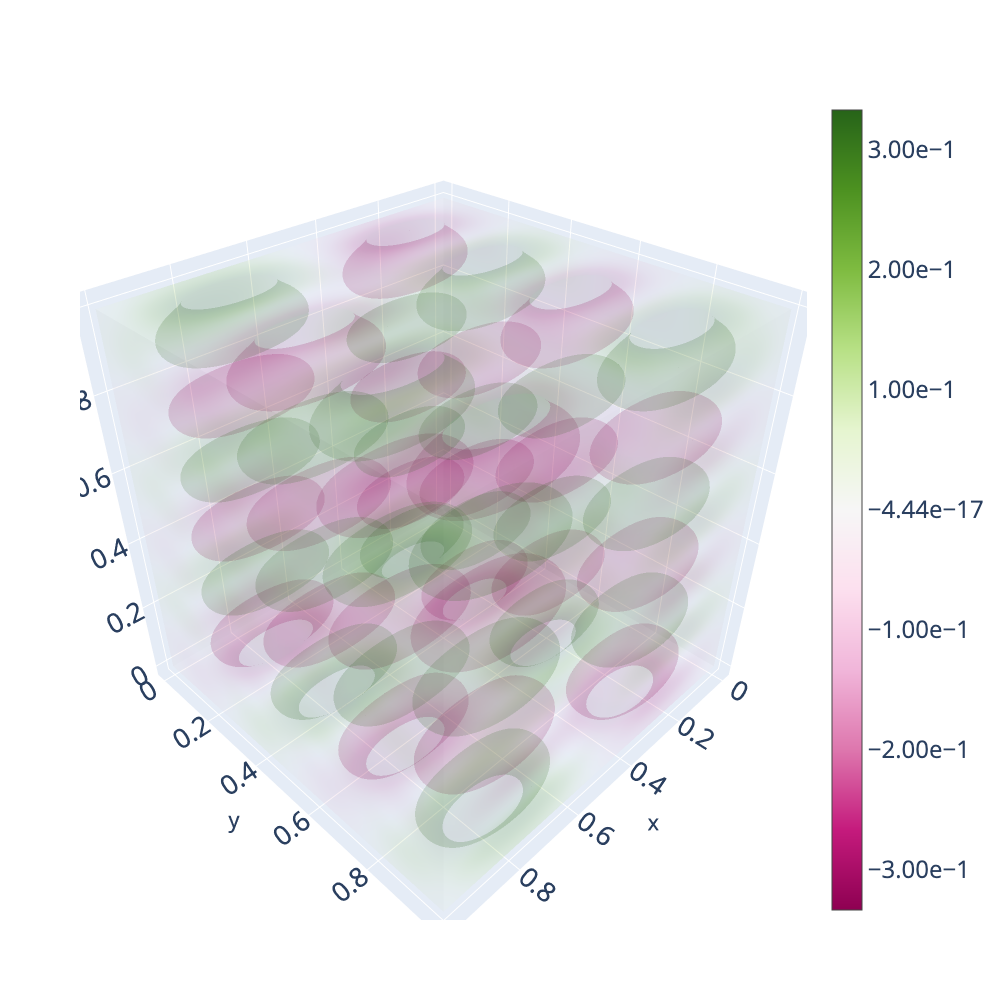
\includegraphics[width=\linewidth]{pictures/10_L1_128_calculated.png}
  \caption{$u_{calculated}$}
\end{subfigure}%
\begin{subfigure}{.33\textwidth}
  \centering
  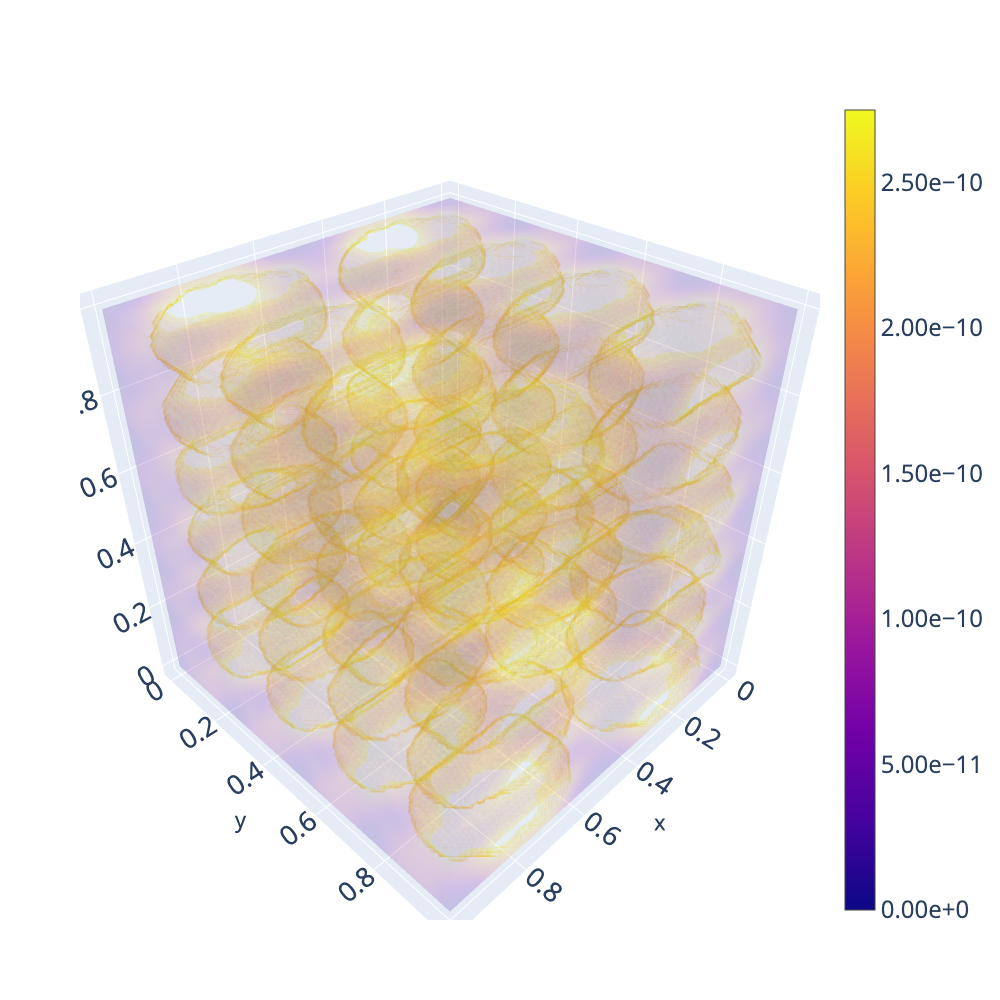
\includegraphics[width=\linewidth]{pictures/10_L1_128_diff.png}
  \caption{погрешность}
\end{subfigure}%
\caption{10 эпоха}
\label{fig:fig}
\end{figure}

\begin{figure}[H]
\begin{subfigure}{.33\textwidth}
  \centering
  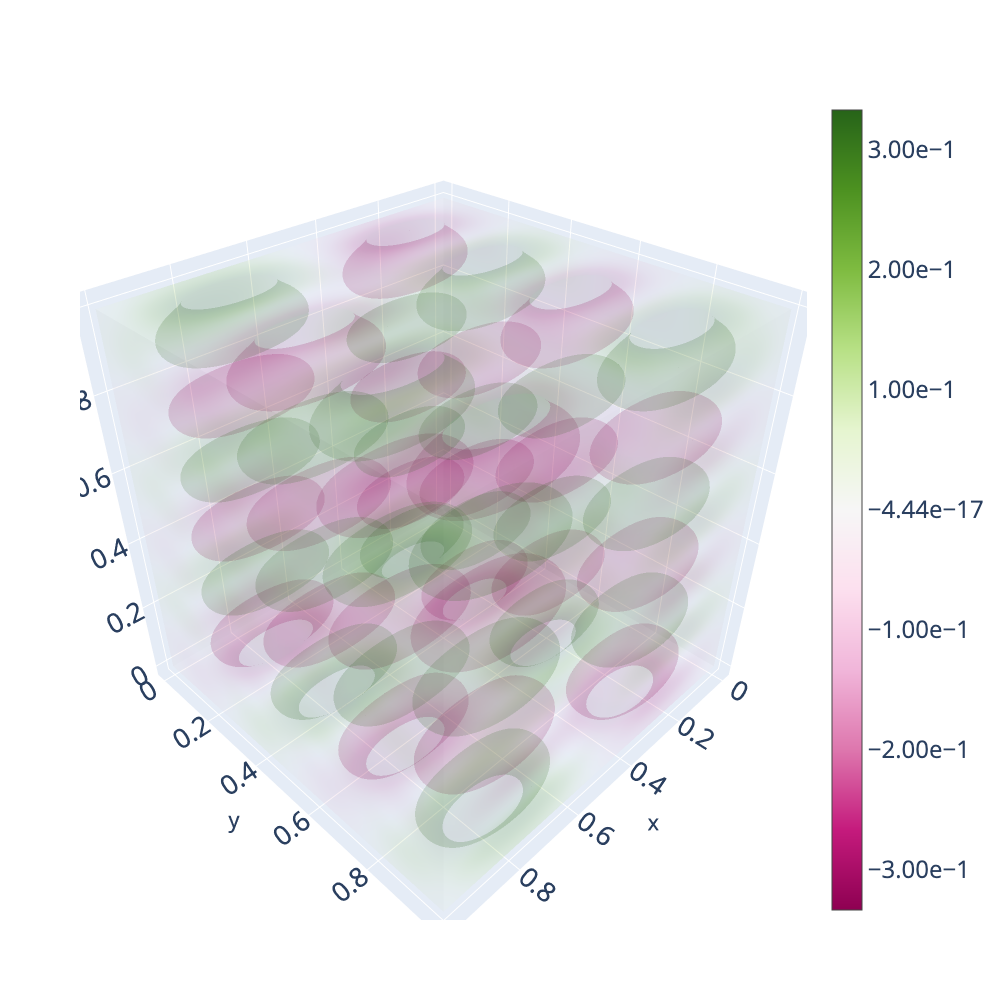
\includegraphics[width=\linewidth]{pictures/19_L1_128_analytical.png}
  \caption{$u_{analytical}$}
\end{subfigure}%
\begin{subfigure}{.33\textwidth}
  \centering
  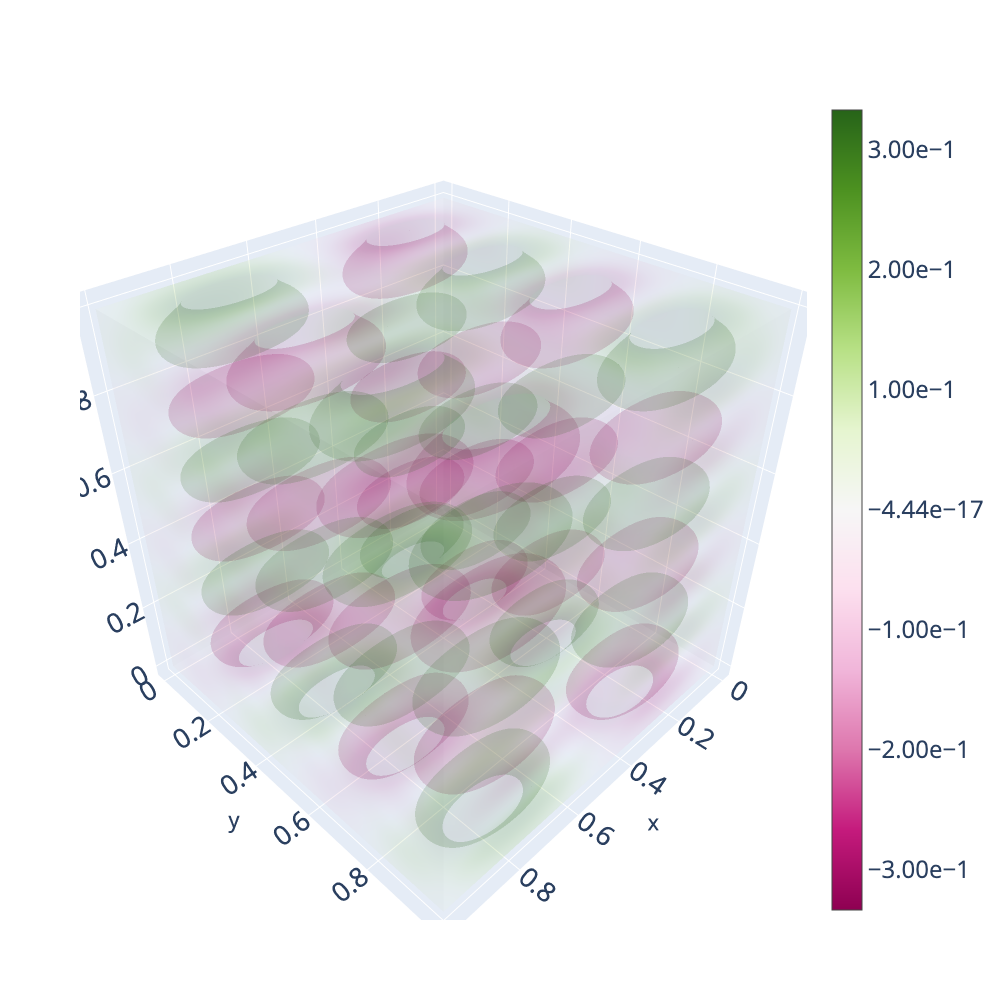
\includegraphics[width=\linewidth]{pictures/19_L1_128_calculated.png}
  \caption{$u_{calculated}$}
\end{subfigure}%
\begin{subfigure}{.33\textwidth}
  \centering
  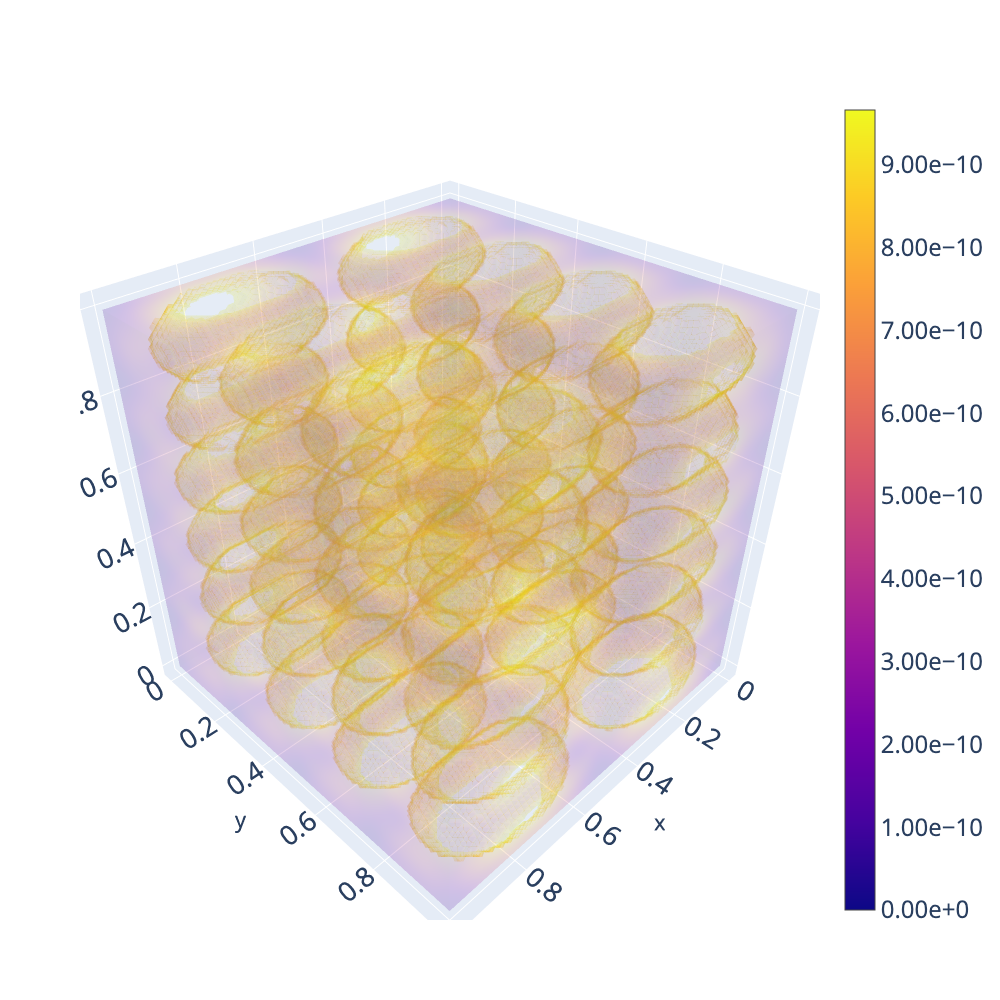
\includegraphics[width=\linewidth]{pictures/19_L1_128_diff.png}
  \caption{погрешность}
\end{subfigure}%
\caption{20 эпоха}
\label{fig:fig}
\end{figure}

\begin{figure}[H]
\begin{subfigure}{.5\textwidth}
  \centering
  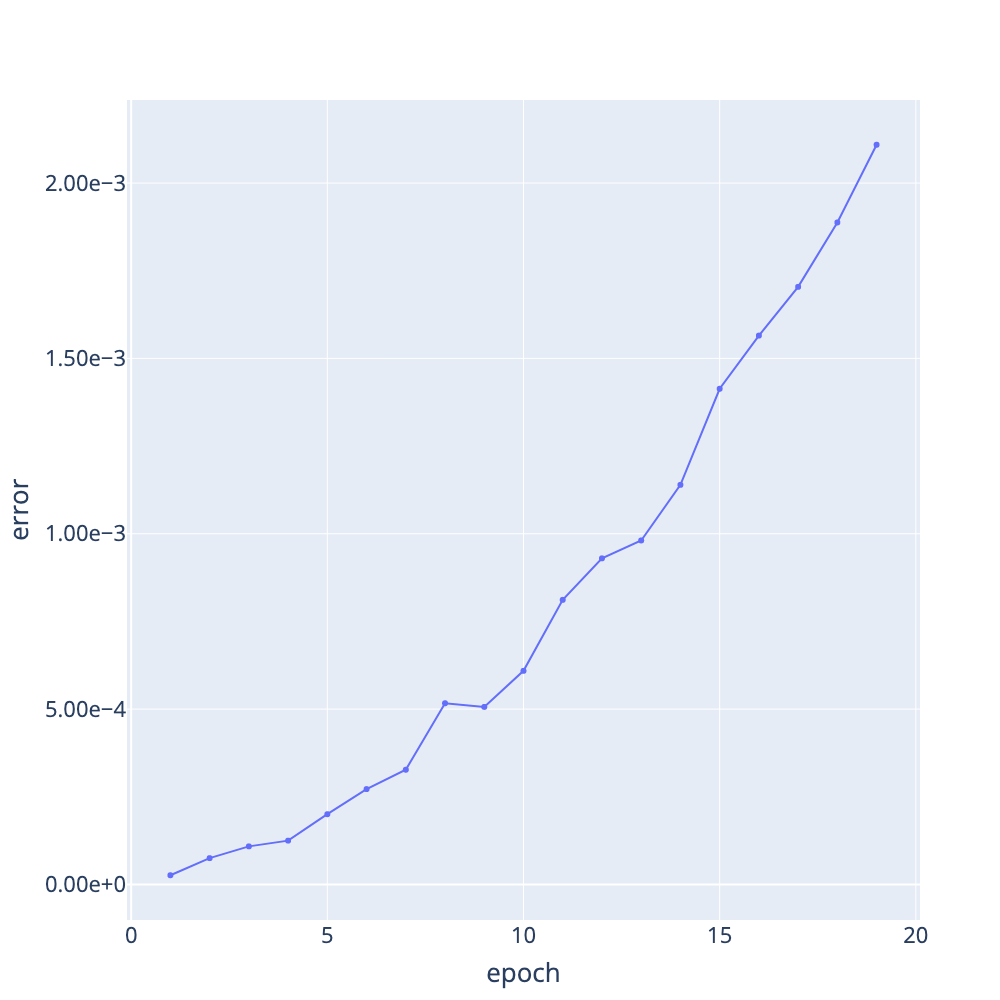
\includegraphics[width=\linewidth]{pictures/L1_128_err.png}
  \caption{Погрешность от эпохи}
\end{subfigure}%
\begin{subfigure}{.5\textwidth}
  \centering
  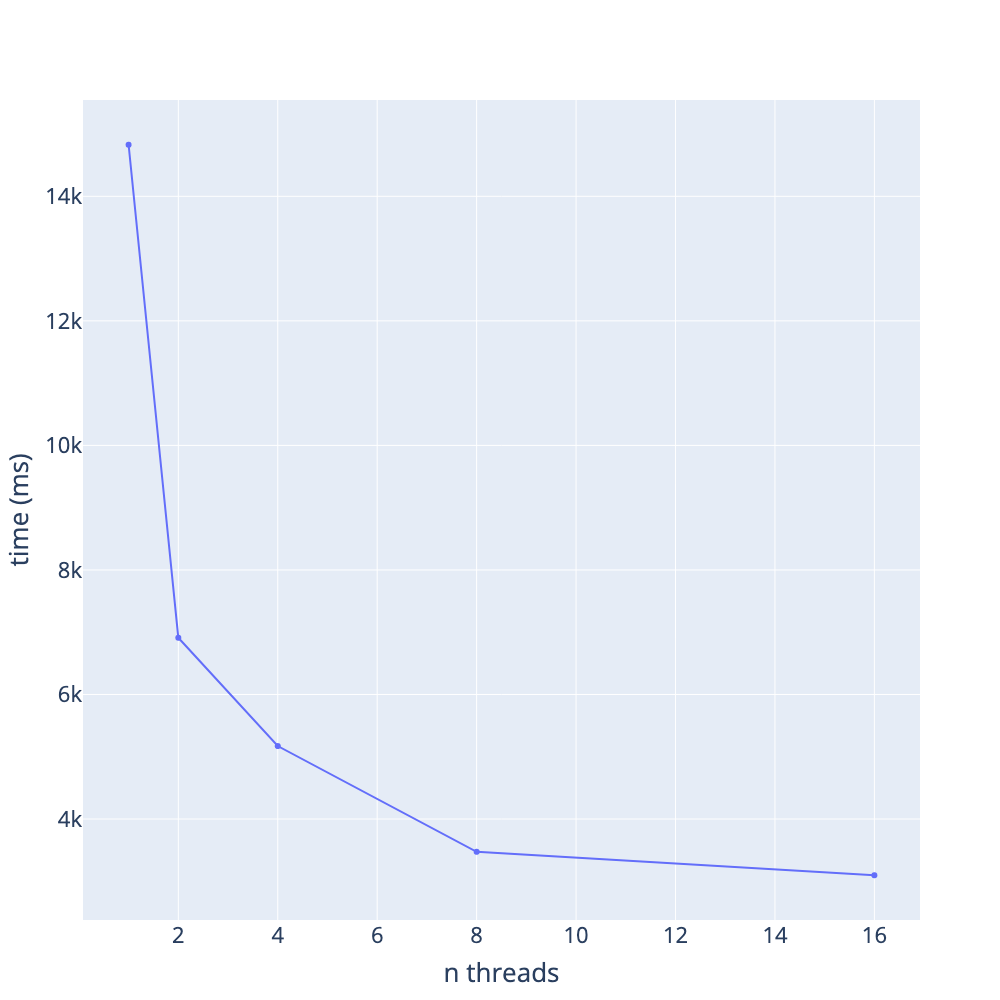
\includegraphics[width=\linewidth]{pictures/L1_128_time_threads.png}
  \caption{Время работы от числа нитей}
\end{subfigure}%
\end{figure}


\subsubsection{Графики для N=256}

\begin{figure}[H]
\begin{subfigure}{.33\textwidth}
  \centering
  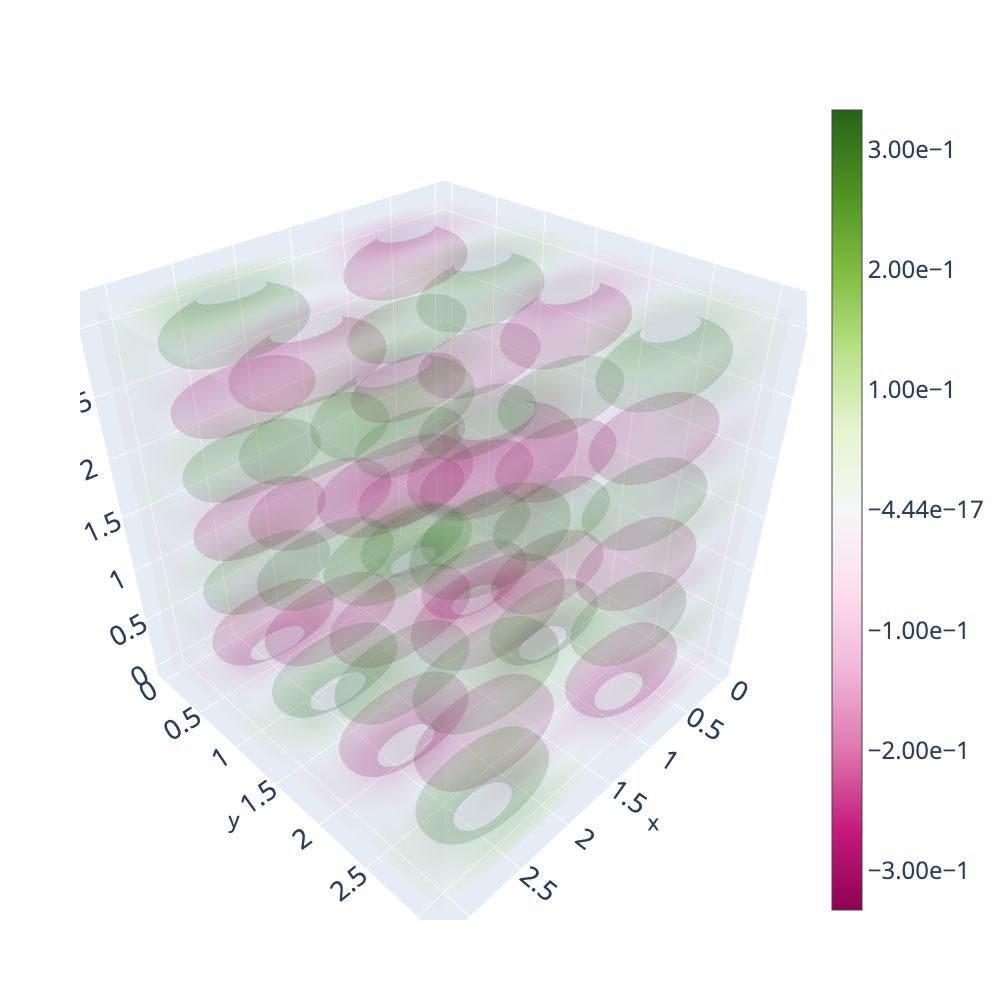
\includegraphics[width=\linewidth]{pictures/1_L1_256_analytical.png}
  \caption{$u_{analytical}$}
\end{subfigure}%
\begin{subfigure}{.33\textwidth}
  \centering
  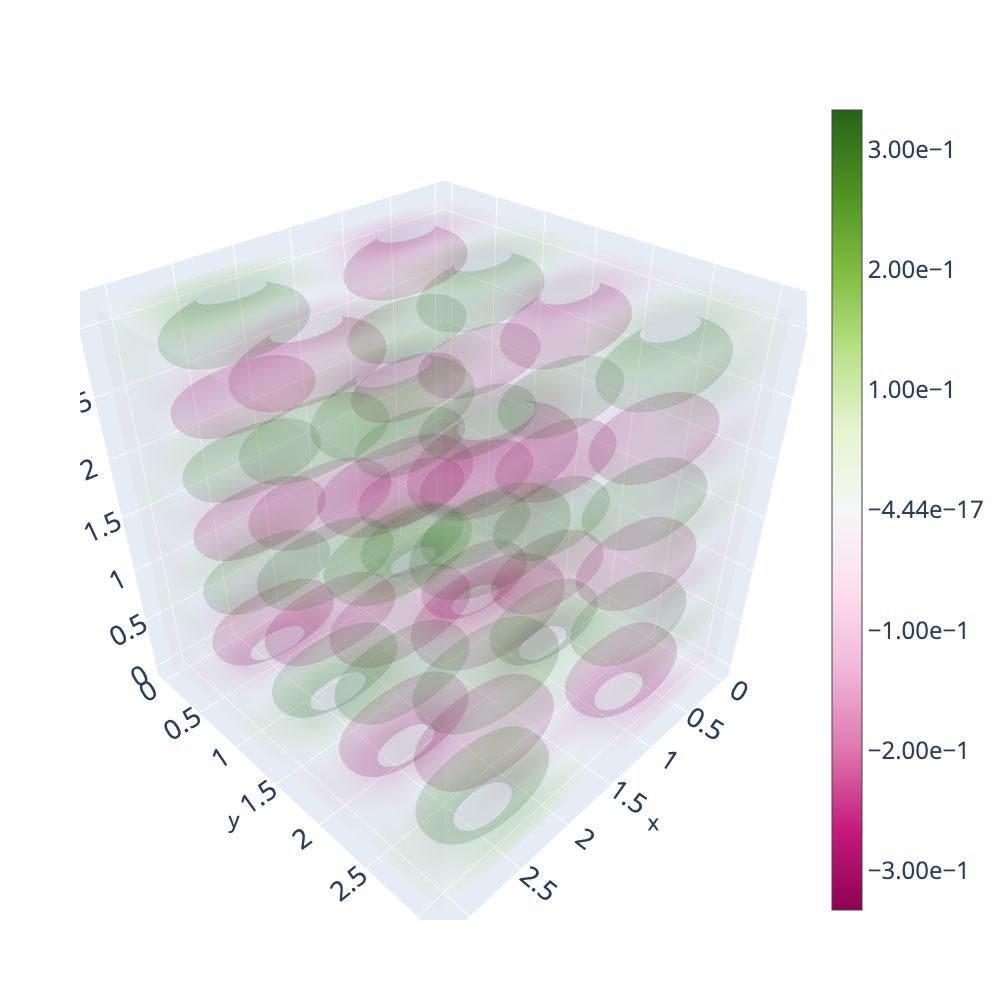
\includegraphics[width=\linewidth]{pictures/1_L1_256_calculated.png}
  \caption{$u_{calculated}$}
\end{subfigure}%
\begin{subfigure}{.33\textwidth}
  \centering
  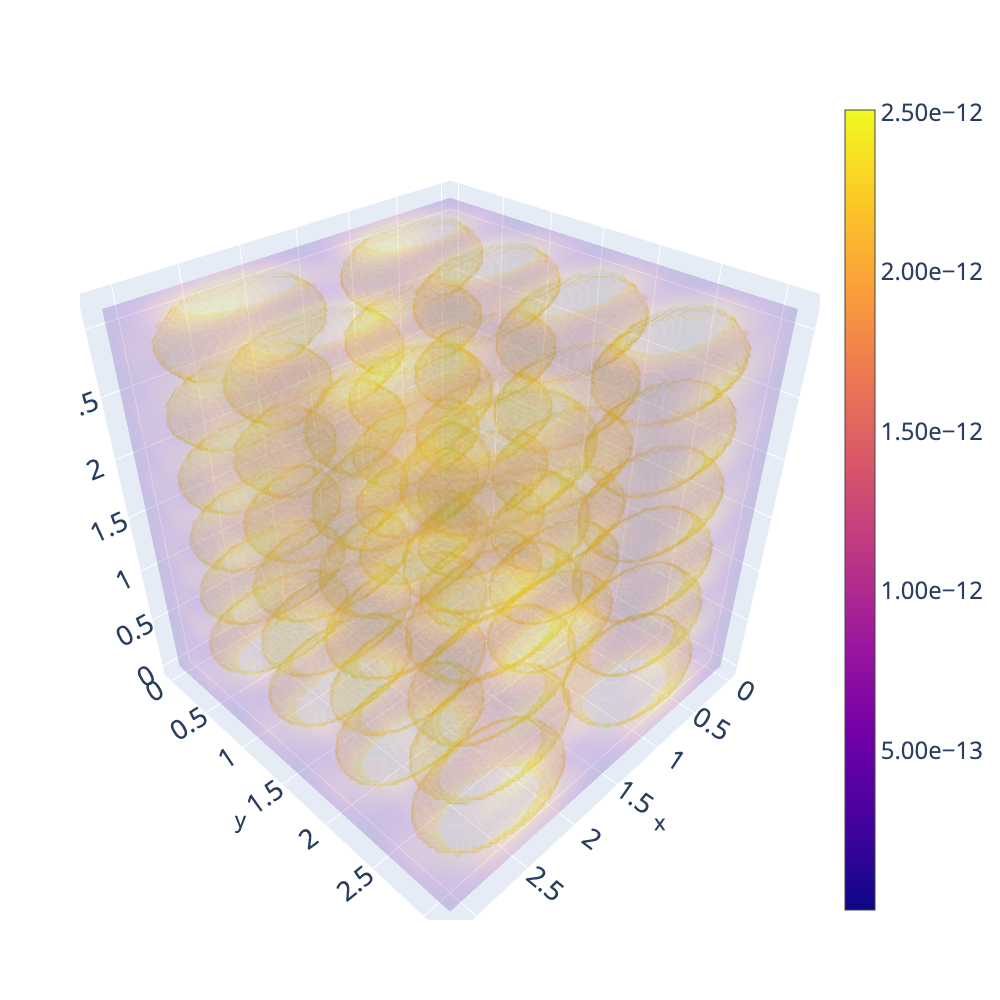
\includegraphics[width=\linewidth]{pictures/1_L1_256_diff.png}
  \caption{погрешность}
\end{subfigure}%
\caption{1 эпоха}
\label{fig:fig}
\end{figure}

\begin{figure}[H]
\begin{subfigure}{.33\textwidth}
  \centering
  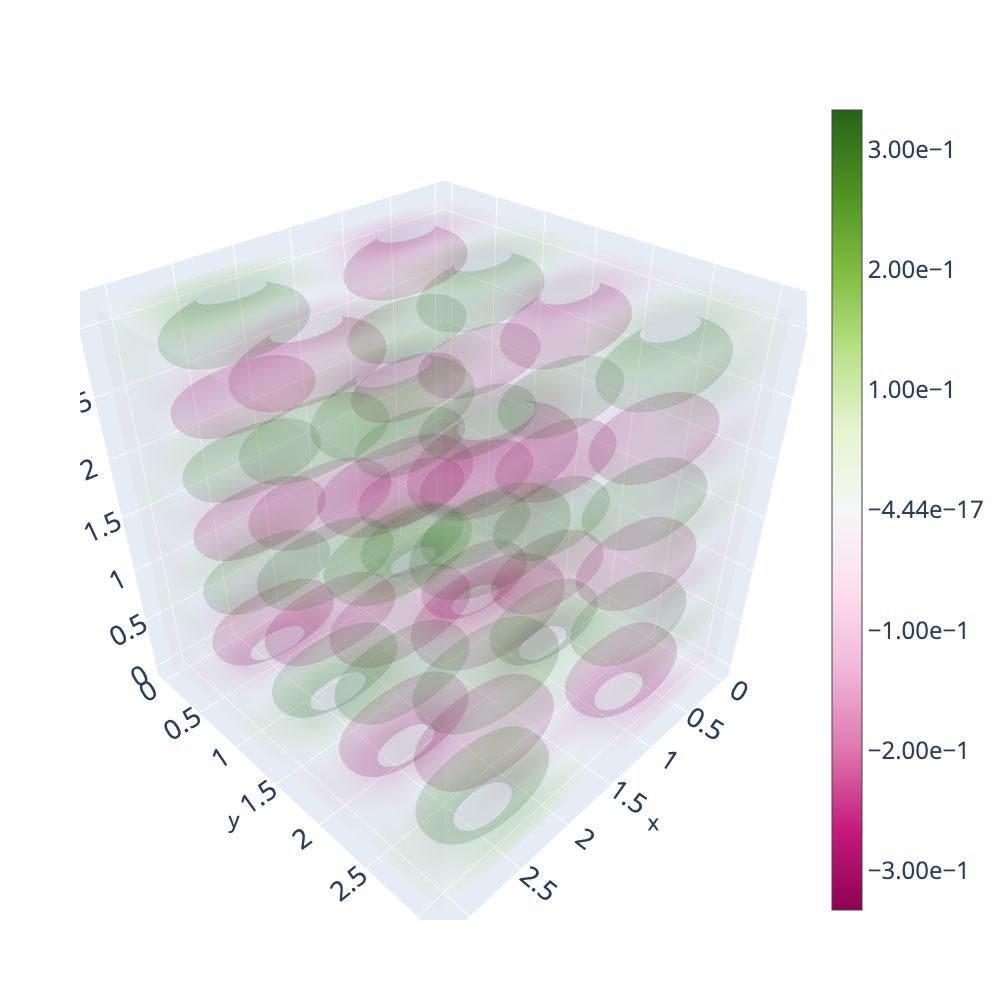
\includegraphics[width=\linewidth]{pictures/10_L1_256_analytical.png}
  \caption{$u_{analytical}$}
\end{subfigure}%
\begin{subfigure}{.33\textwidth}
  \centering
  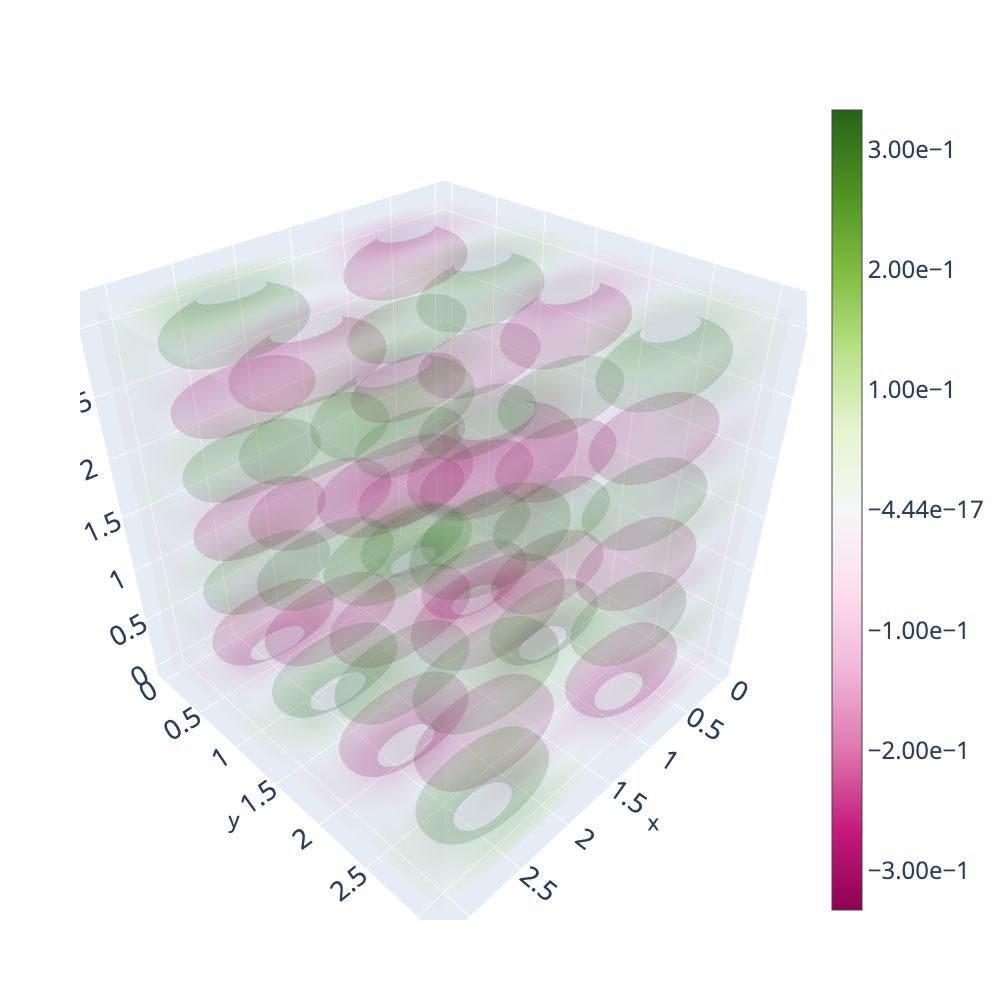
\includegraphics[width=\linewidth]{pictures/10_L1_256_calculated.png}
  \caption{$u_{calculated}$}
\end{subfigure}%
\begin{subfigure}{.33\textwidth}
  \centering
  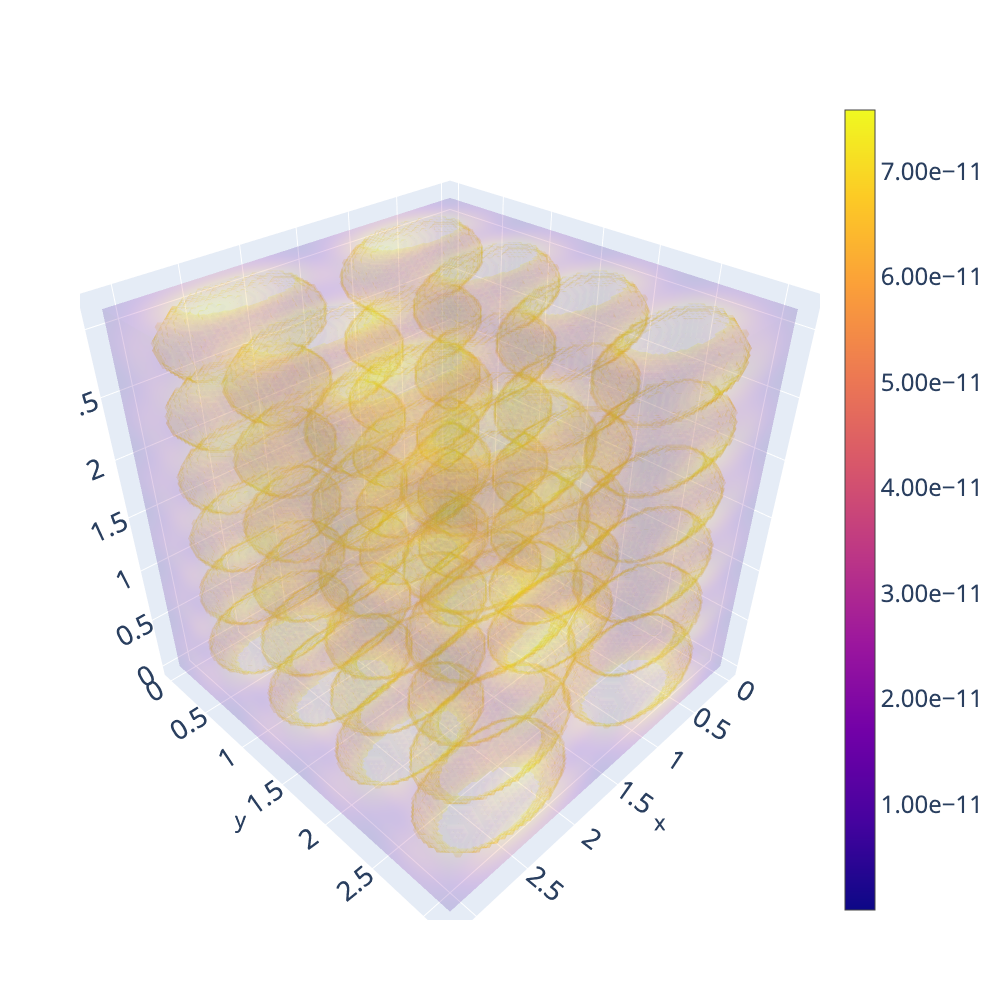
\includegraphics[width=\linewidth]{pictures/10_L1_256_diff.png}
  \caption{погрешность}
\end{subfigure}%
\caption{10 эпоха}
\label{fig:fig}
\end{figure}

\begin{figure}[H]
\begin{subfigure}{.33\textwidth}
  \centering
  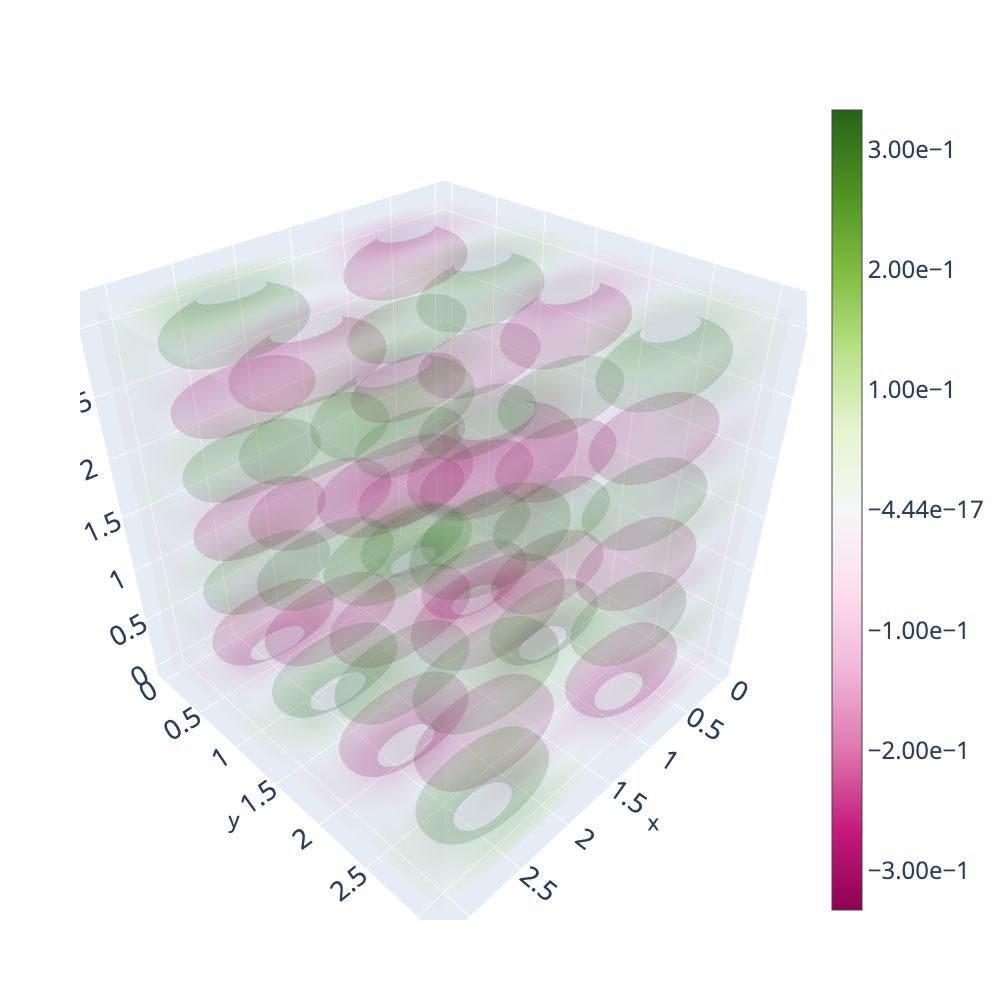
\includegraphics[width=\linewidth]{pictures/19_L1_256_analytical.png}
  \caption{$u_{analytical}$}
\end{subfigure}%
\begin{subfigure}{.33\textwidth}
  \centering
  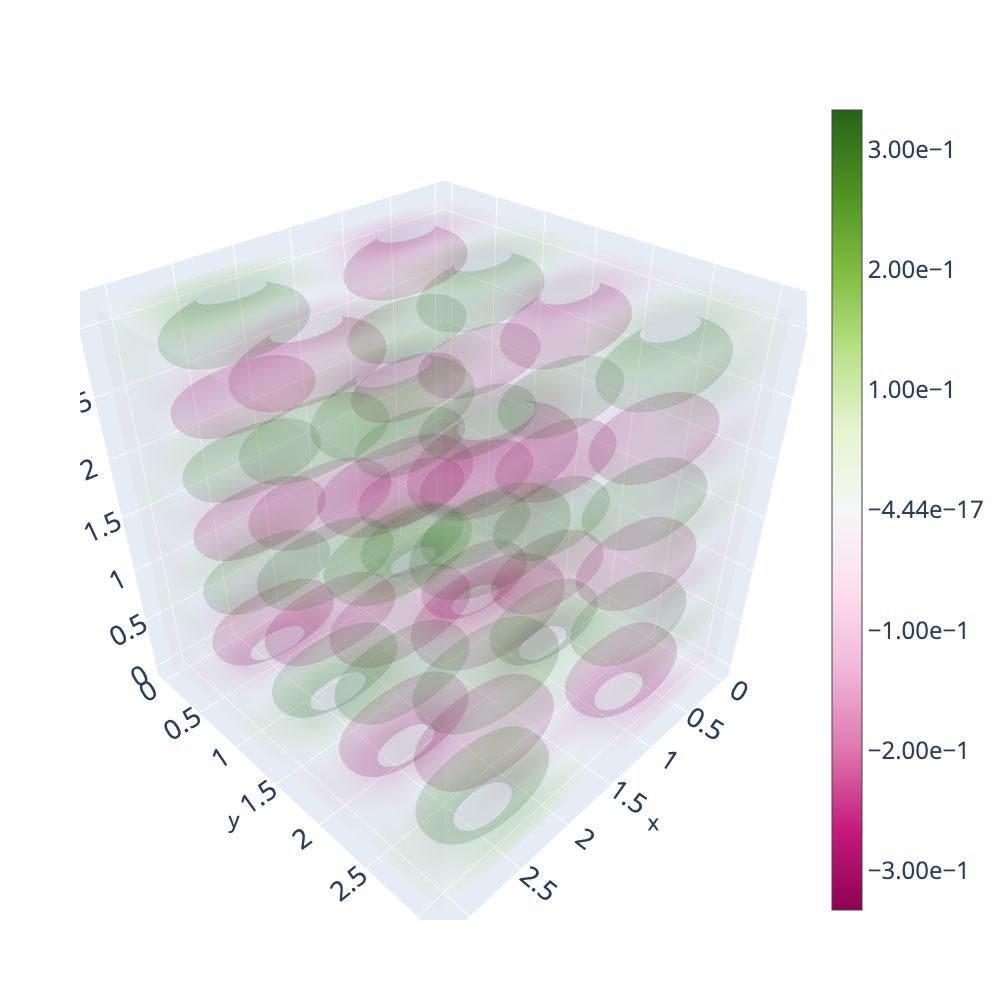
\includegraphics[width=\linewidth]{pictures/19_L1_256_calculated.png}
  \caption{$u_{calculated}$}
\end{subfigure}%
\begin{subfigure}{.33\textwidth}
  \centering
  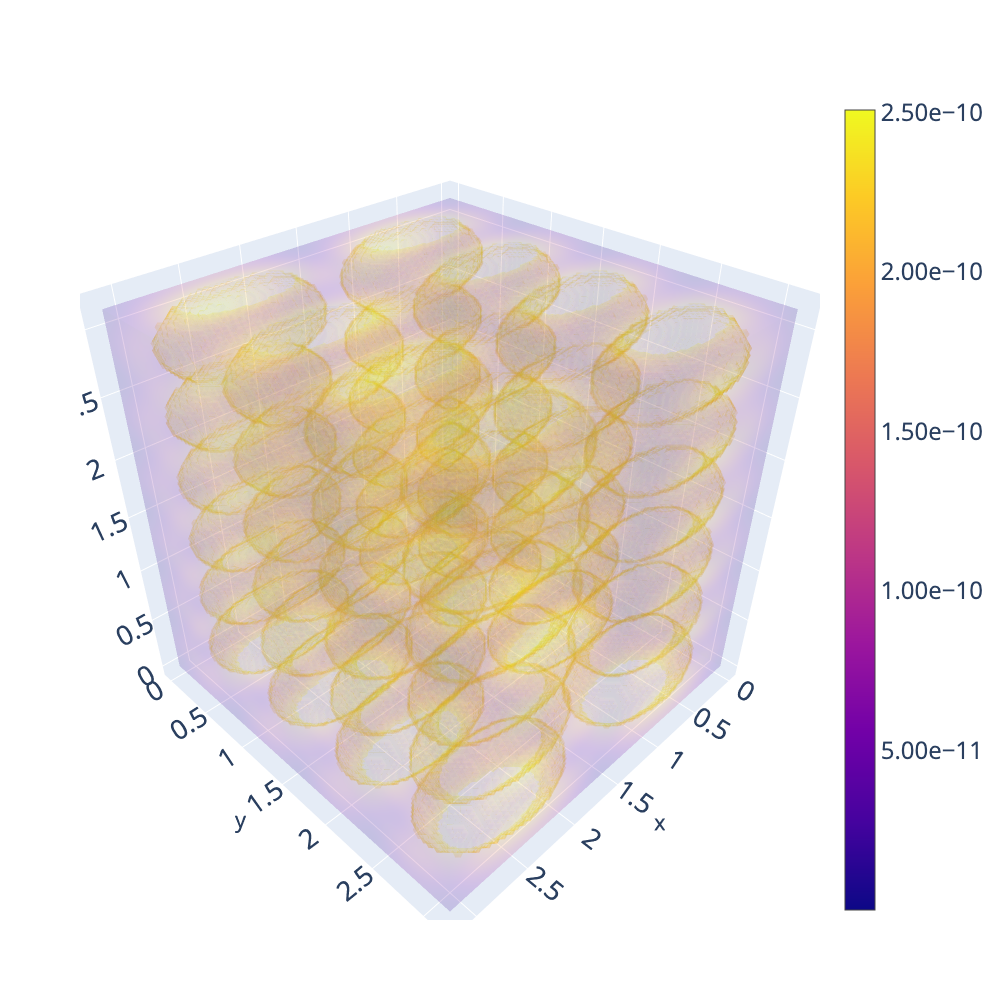
\includegraphics[width=\linewidth]{pictures/19_L1_256_diff.png}
  \caption{погрешность}
\end{subfigure}%
\caption{20 эпоха}
\label{fig:fig}
\end{figure}

\begin{figure}[H]
\begin{subfigure}{.5\textwidth}
  \centering
  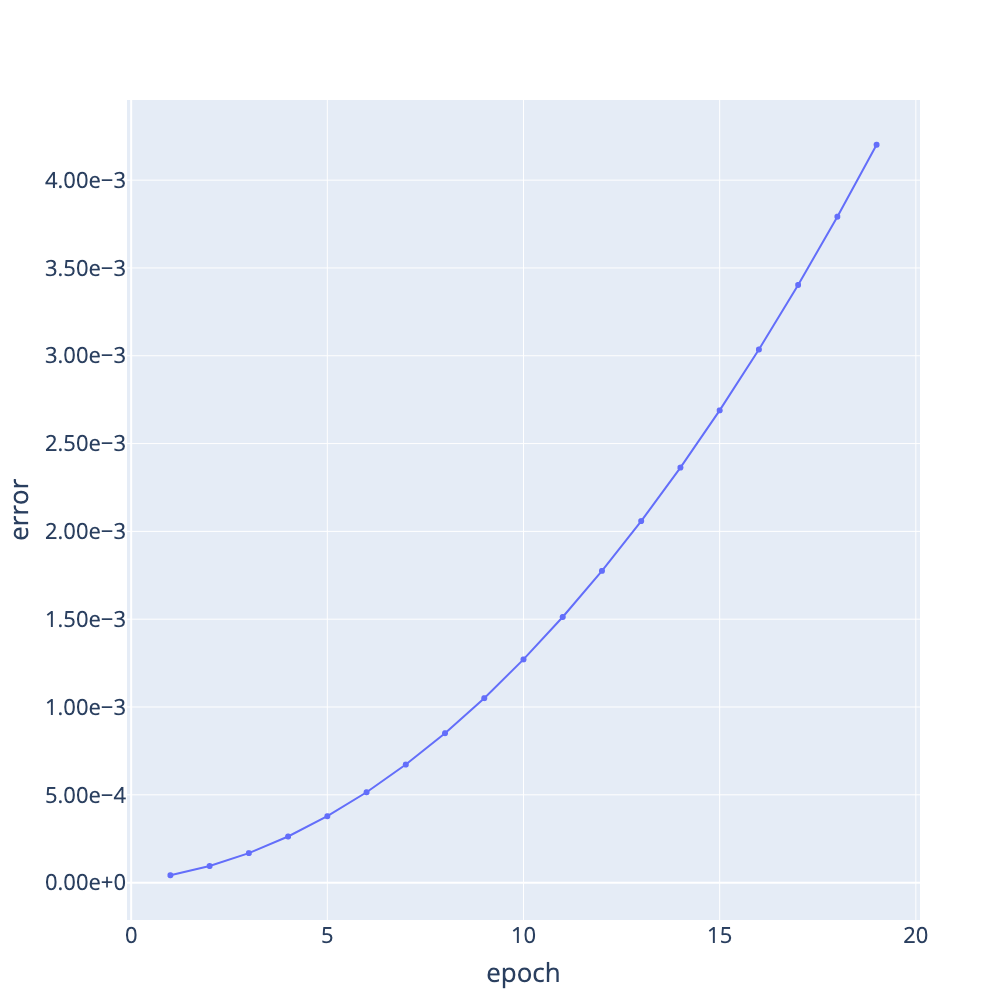
\includegraphics[width=\linewidth]{pictures/L1_256_err.png}
  \caption{Погрешность от эпохи}
\end{subfigure}%
\begin{subfigure}{.5\textwidth}
  \centering
  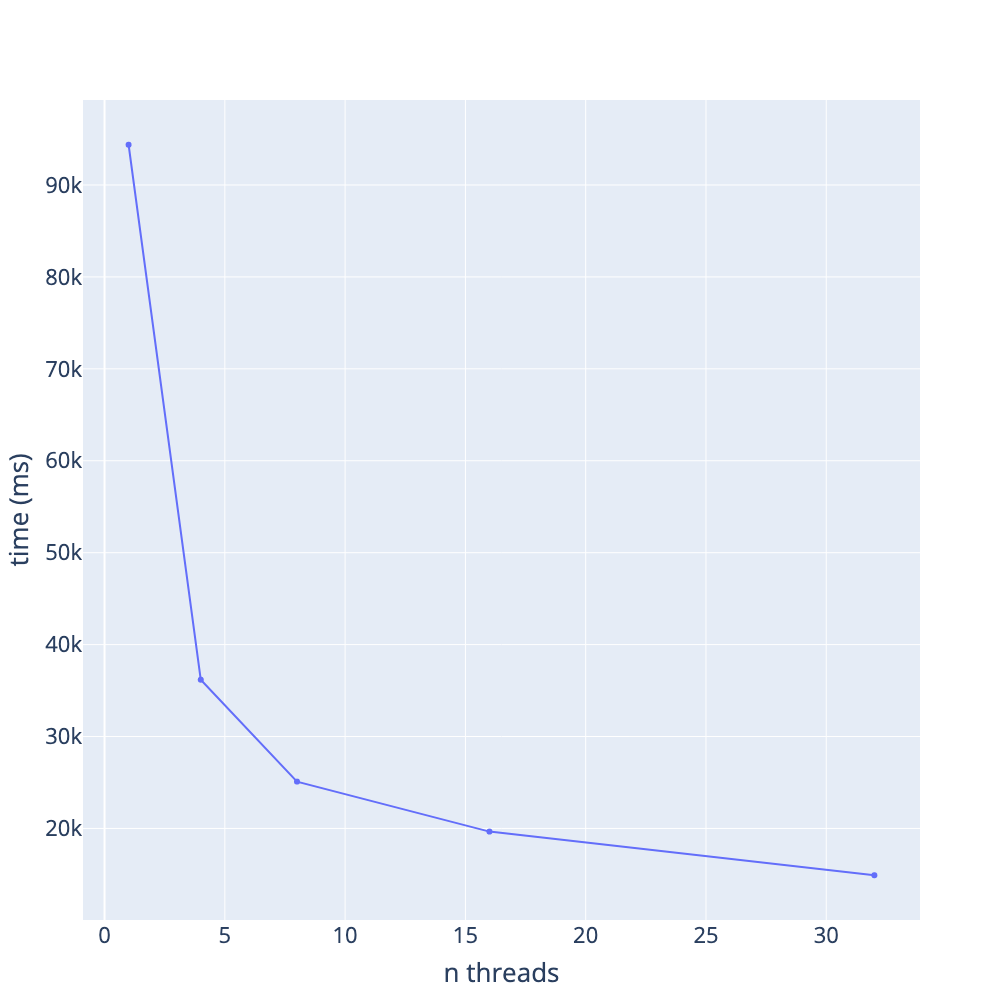
\includegraphics[width=\linewidth]{pictures/L1_256_time_threads.png}
  \caption{Время работы от числа нитей}
\end{subfigure}%
\end{figure}

\newpage
\subsection{L = $\pi$}

{
\centering
\noindent\begin{tabular}{|p{2cm}|p{2.5cm}|p{2.5cm}|p{2cm}|p{3cm}|}
    \hline
    \textit{Число OpenMP нитей} & \textit{Число точек сетки }$N^3$ & \textit{Время решения T (ms)} & \textit{Ускорение S} & \textit{Погрешность }$\delta$ \\
    \hline
    1 & $128^3$ & 13009.1 & 1 & 0.000212559 \\
    2 & $128^3$ & 9545.68 & 1.36 & 0.000212559 \\
    4 & $128^3$ & 5383.07 & 2.42 & 0.000212559 \\
    8 & $128^3$ & 4221.77 & 3.08 & 0.000212559 \\
    16 & $128^3$ & 3620.54 & 3.59 & 0.000212559 \\
    \hline
    1 & $256^3$ & 98665.7 & 1 & 0.00042571 \\
    4 & $256^3$ & 37394.8 & 2.64 & 0.00042571 \\
    8 & $256^3$ & 24504.9 & 4.03 & 0.00042571 \\
    16 & $256^3$ & 19678.3 & 5.01 & 0.00042571 \\
    32 & $256^3$ & 16161.1 & 6.11 & 0.00042571 \\
    \hline
\end{tabular}
}

\subsubsection{Графики для N=128}

\begin{figure}[H]
\begin{subfigure}{.33\textwidth}
  \centering
  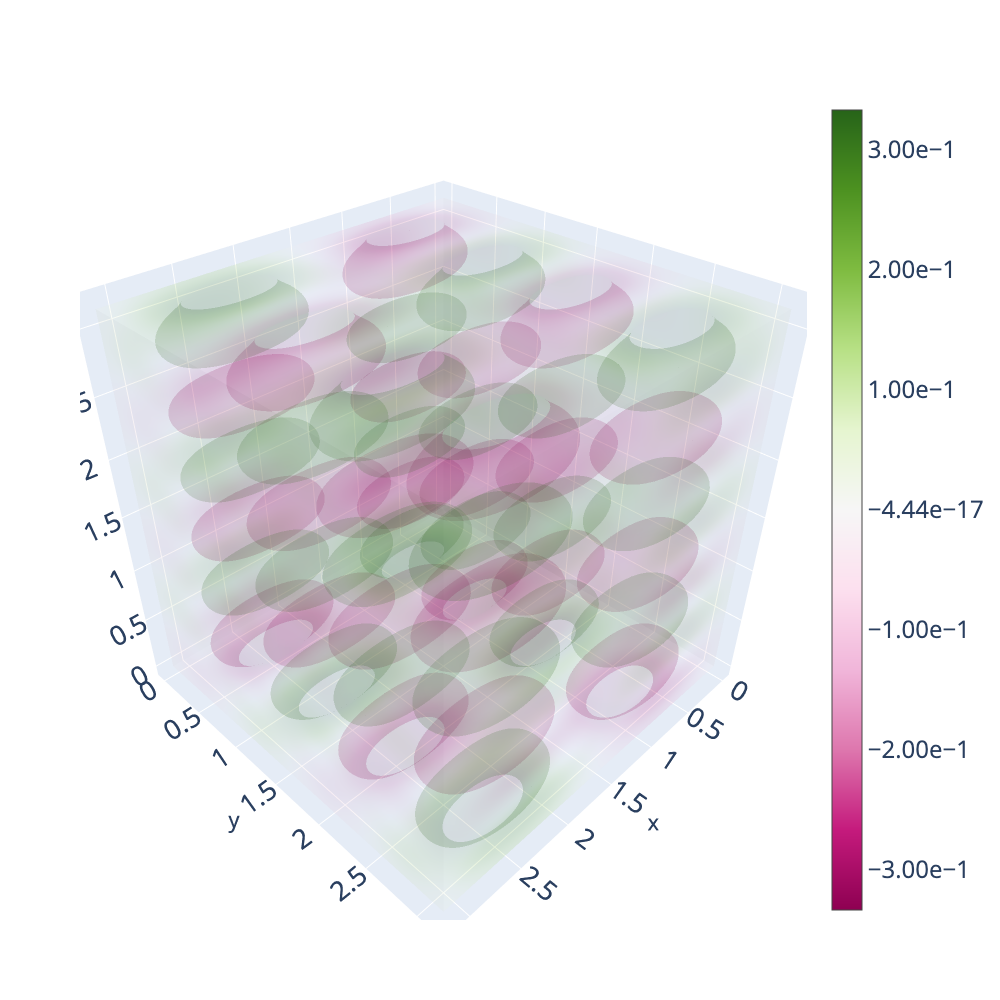
\includegraphics[width=\linewidth]{pictures/1_Lpi_128_analytical.png}
  \caption{$u_{analytical}$}
\end{subfigure}%
\begin{subfigure}{.33\textwidth}
  \centering
  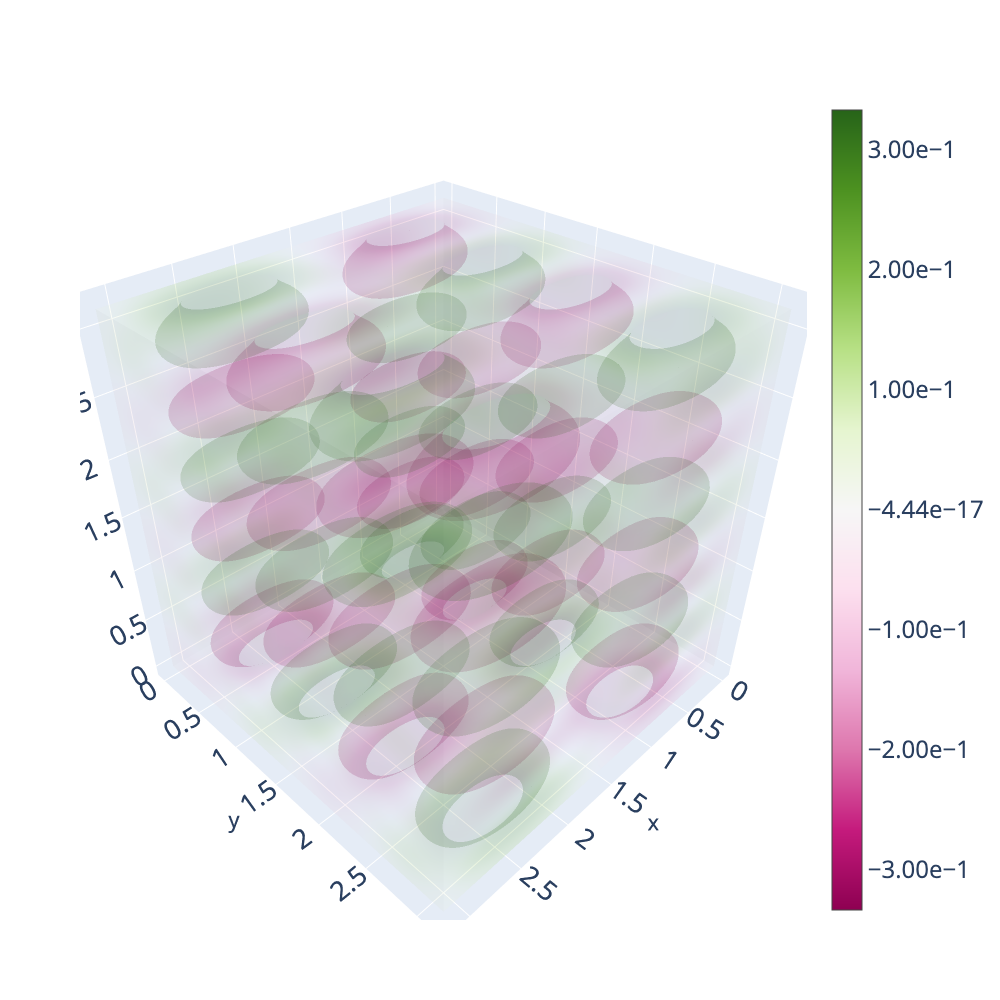
\includegraphics[width=\linewidth]{pictures/1_Lpi_128_calculated.png}
  \caption{$u_{calculated}$}
\end{subfigure}%
\begin{subfigure}{.33\textwidth}
  \centering
  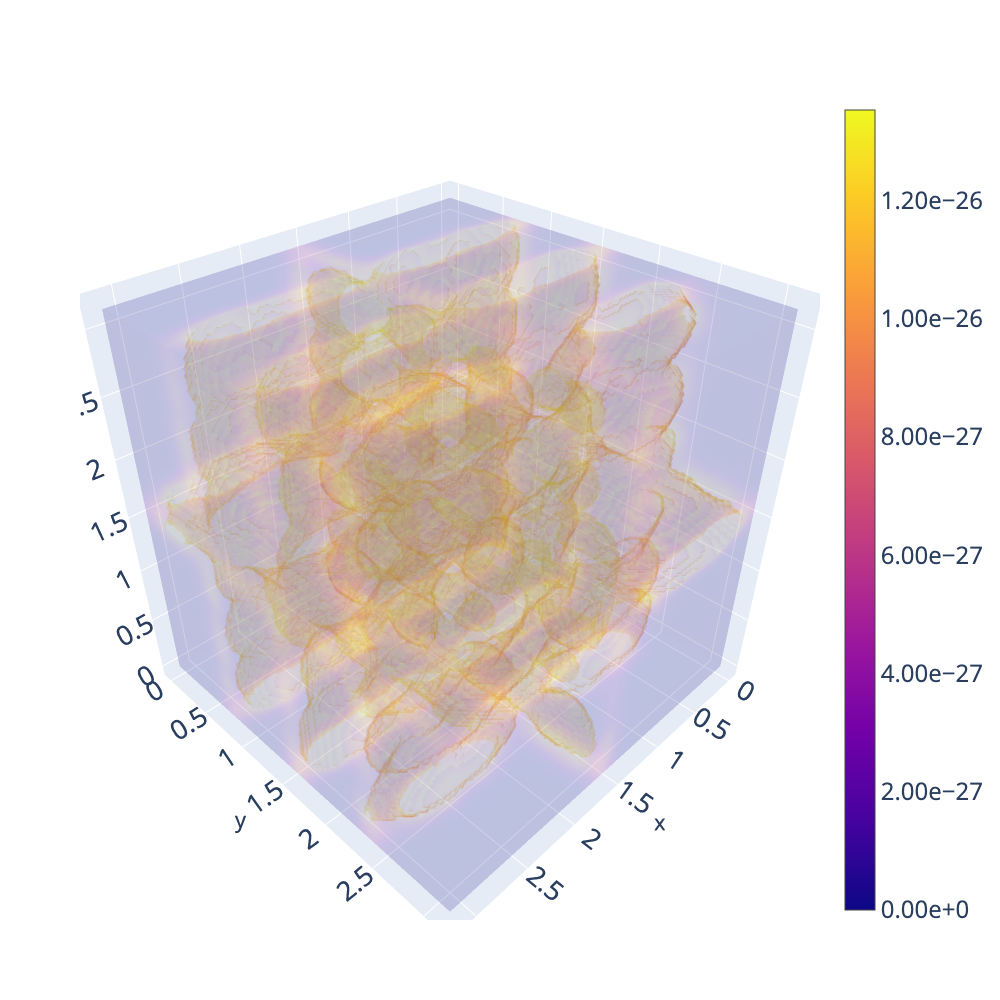
\includegraphics[width=\linewidth]{pictures/1_Lpi_128_diff.png}
  \caption{погрешность}
\end{subfigure}%
\caption{1 эпоха}
\label{fig:fig}
\end{figure}

\begin{figure}[H]
\begin{subfigure}{.33\textwidth}
  \centering
  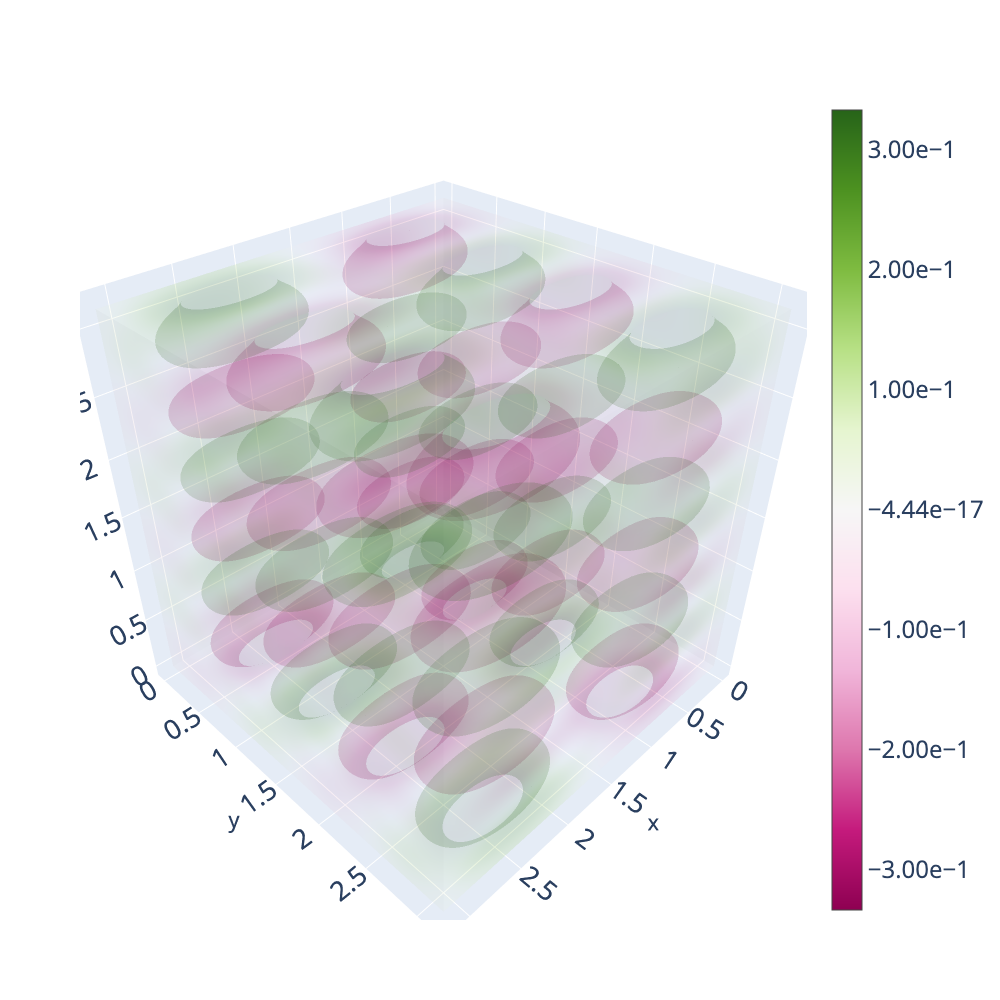
\includegraphics[width=\linewidth]{pictures/10_Lpi_128_analytical.png}
  \caption{$u_{analytical}$}
\end{subfigure}%
\begin{subfigure}{.33\textwidth}
  \centering
  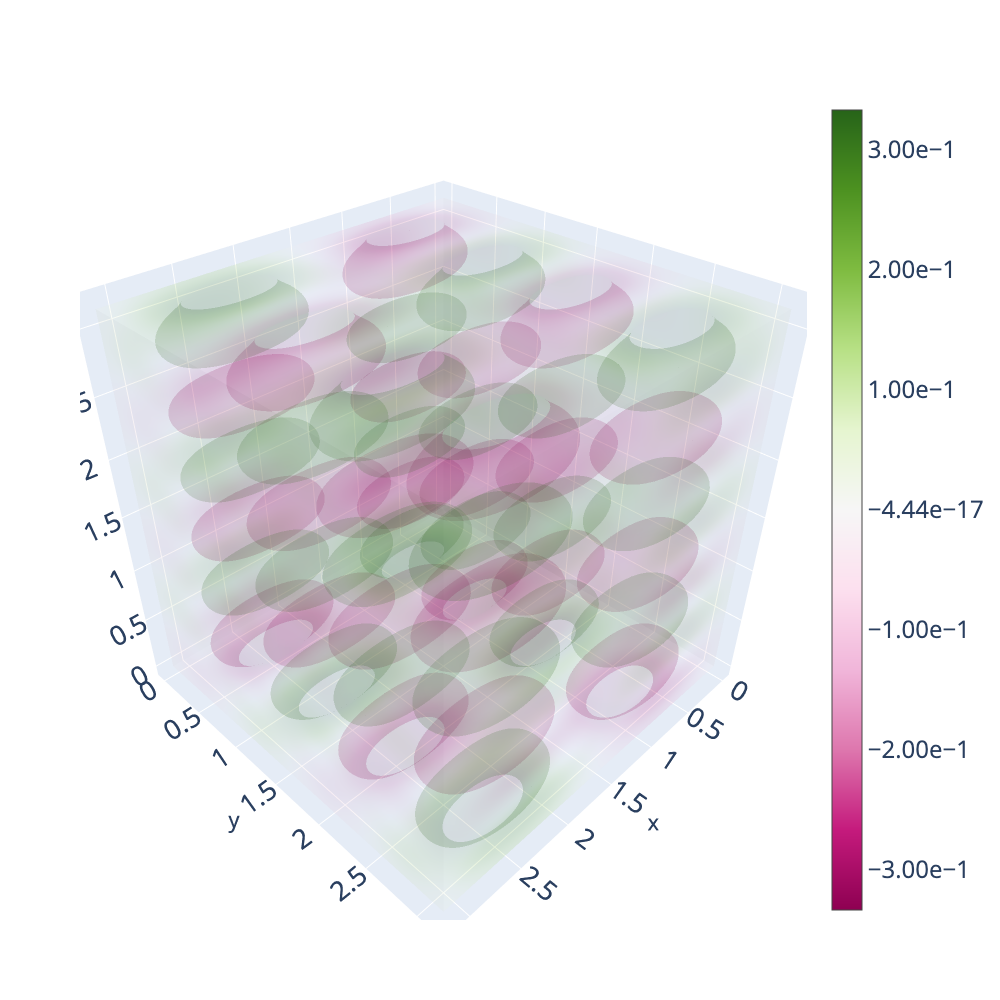
\includegraphics[width=\linewidth]{pictures/10_Lpi_128_calculated.png}
  \caption{$u_{calculated}$}
\end{subfigure}%
\begin{subfigure}{.33\textwidth}
  \centering
  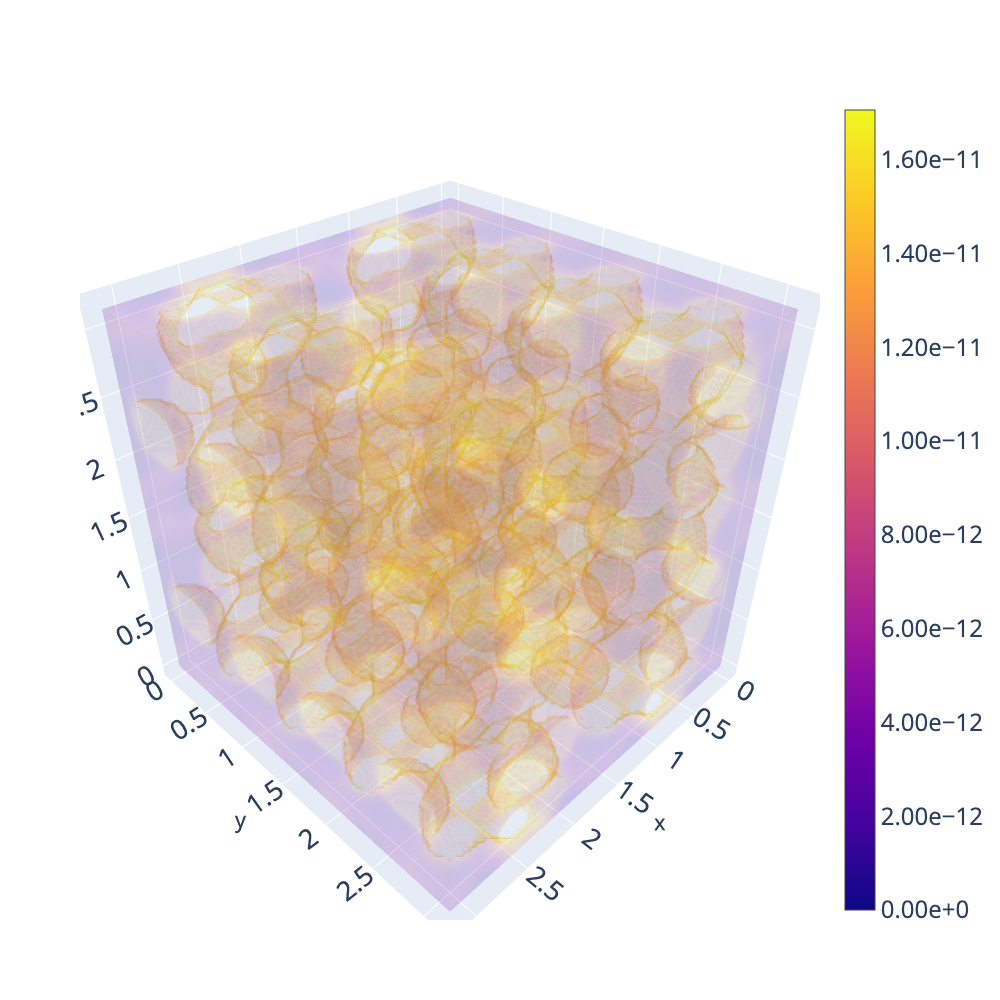
\includegraphics[width=\linewidth]{pictures/10_Lpi_128_diff.png}
  \caption{погрешность}
\end{subfigure}%
\caption{10 эпоха}
\label{fig:fig}
\end{figure}

\begin{figure}[H]
\begin{subfigure}{.33\textwidth}
  \centering
  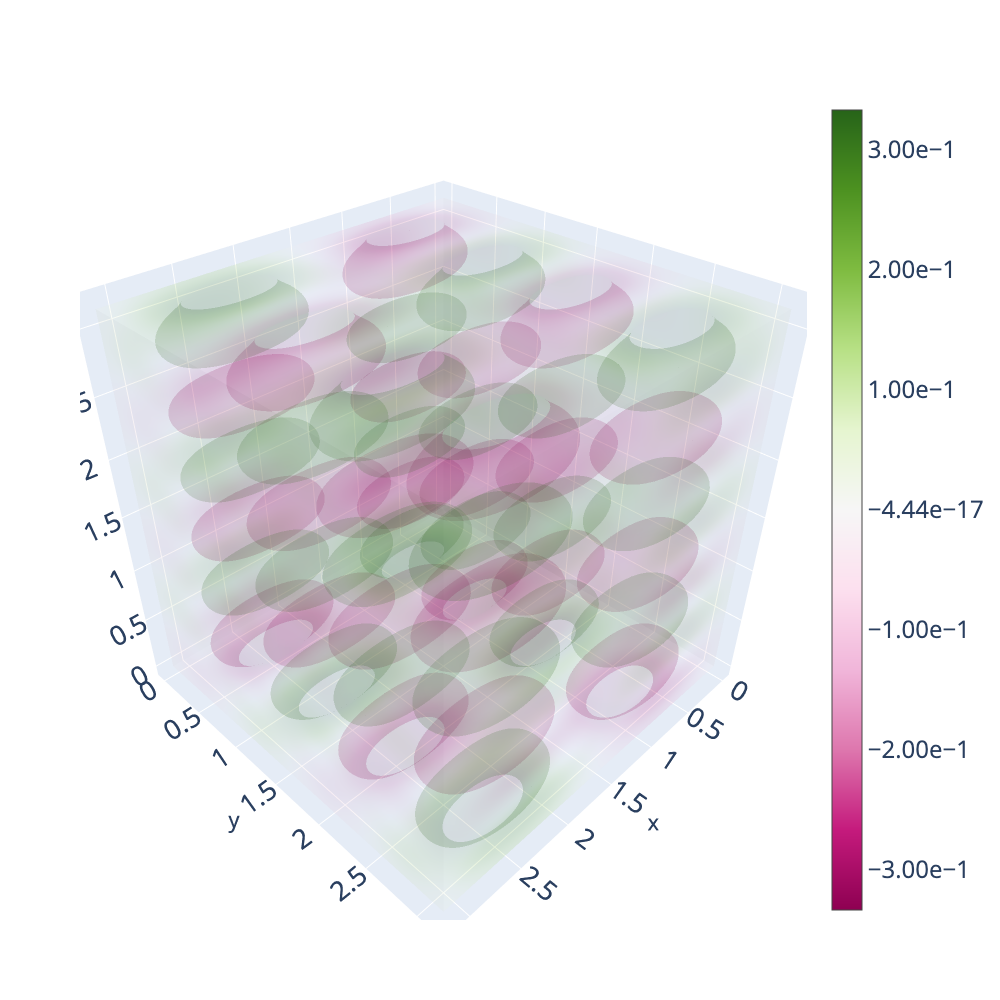
\includegraphics[width=\linewidth]{pictures/19_Lpi_128_analytical.png}
  \caption{$u_{analytical}$}
\end{subfigure}%
\begin{subfigure}{.33\textwidth}
  \centering
  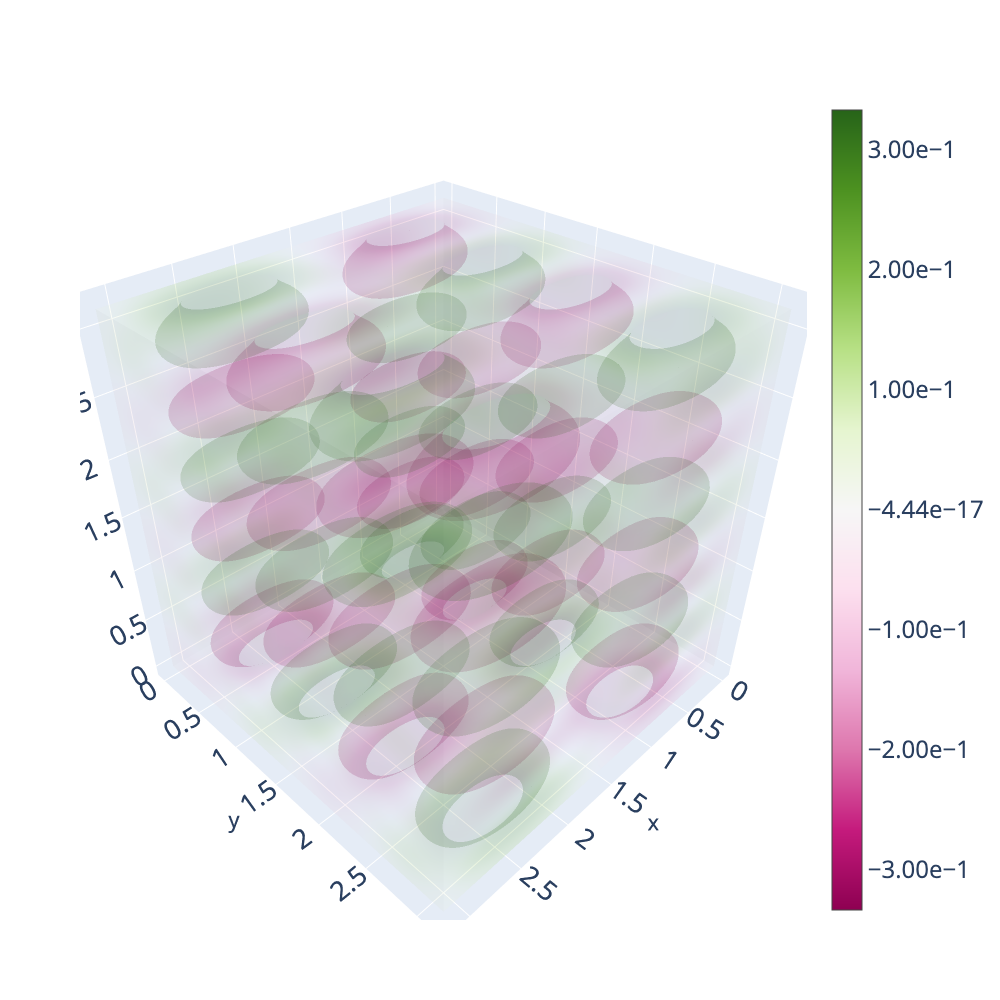
\includegraphics[width=\linewidth]{pictures/19_Lpi_128_calculated.png}
  \caption{$u_{calculated}$}
\end{subfigure}%
\begin{subfigure}{.33\textwidth}
  \centering
  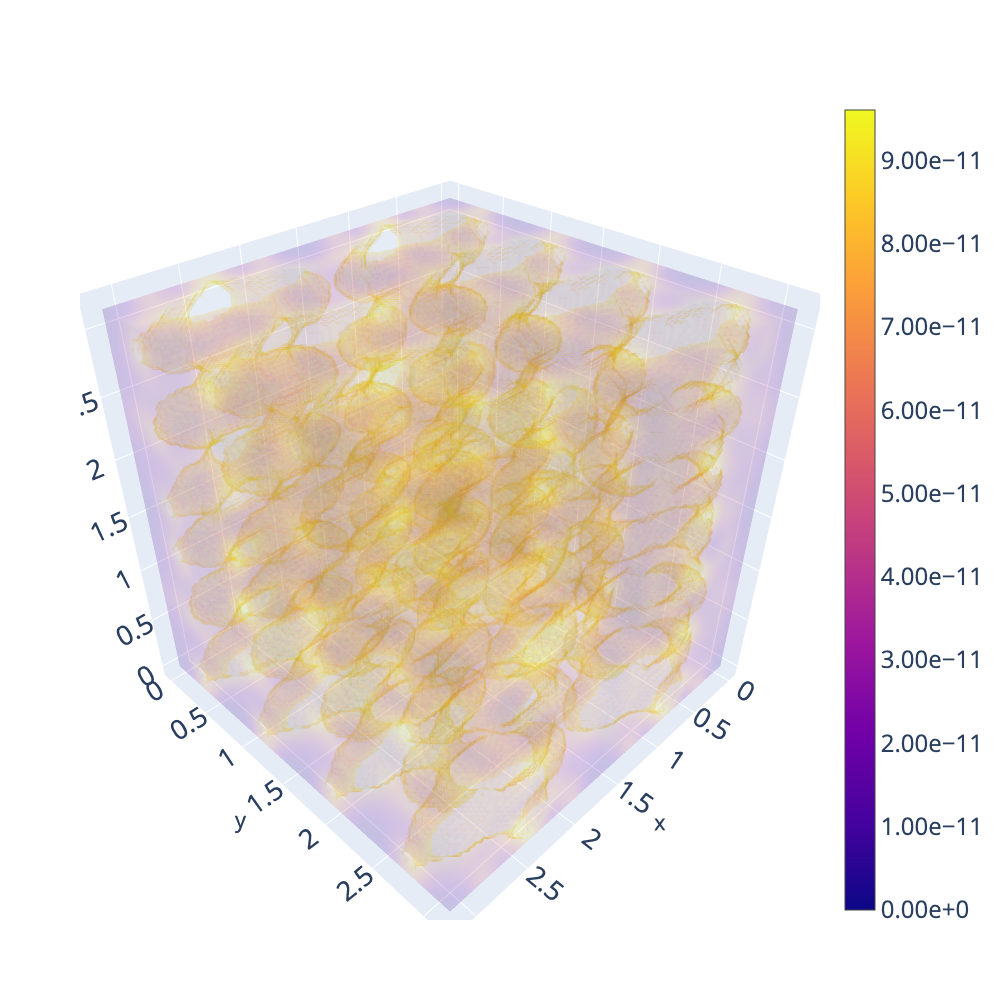
\includegraphics[width=\linewidth]{pictures/19_Lpi_128_diff.png}
  \caption{погрешность}
\end{subfigure}%
\caption{20 эпоха}
\label{fig:fig}
\end{figure}

\begin{figure}[H]
\begin{subfigure}{.5\textwidth}
  \centering
  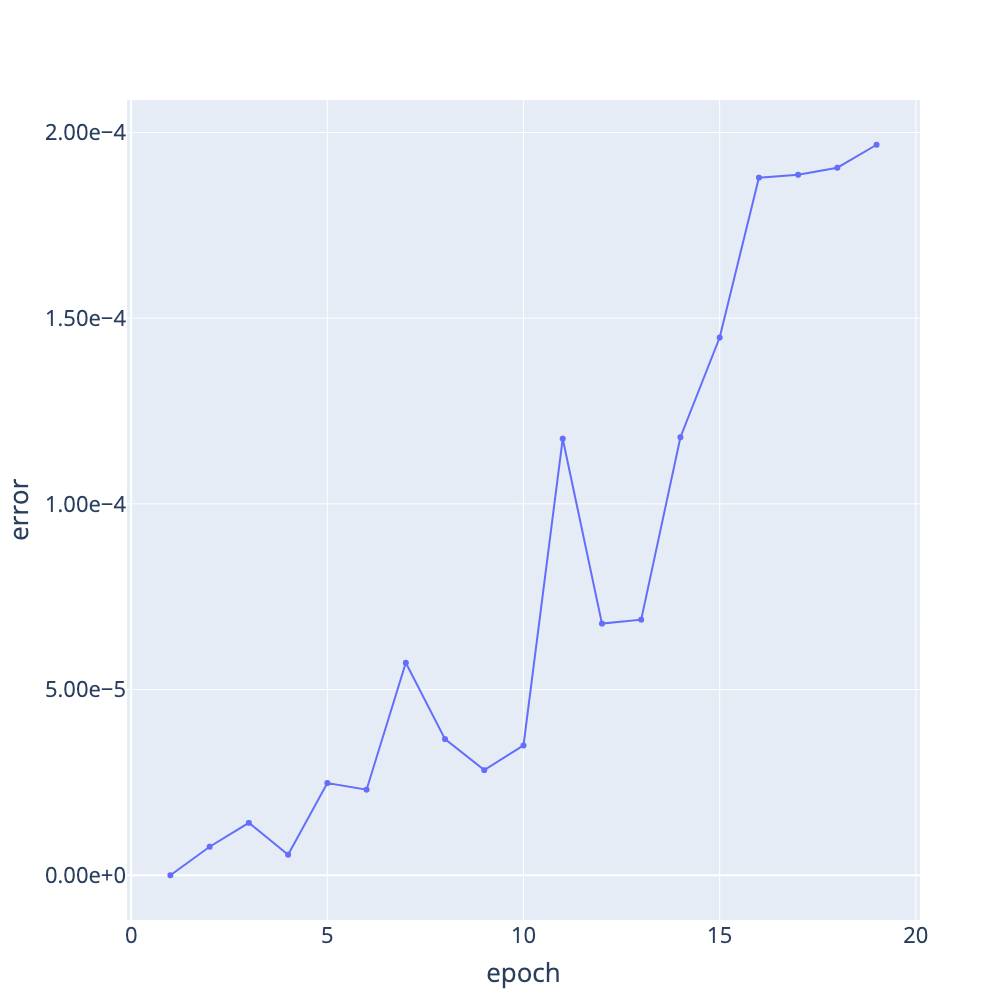
\includegraphics[width=\linewidth]{pictures/Lpi_128_err.png}
  \caption{Погрешность от эпохи}
\end{subfigure}%
\begin{subfigure}{.5\textwidth}
  \centering
  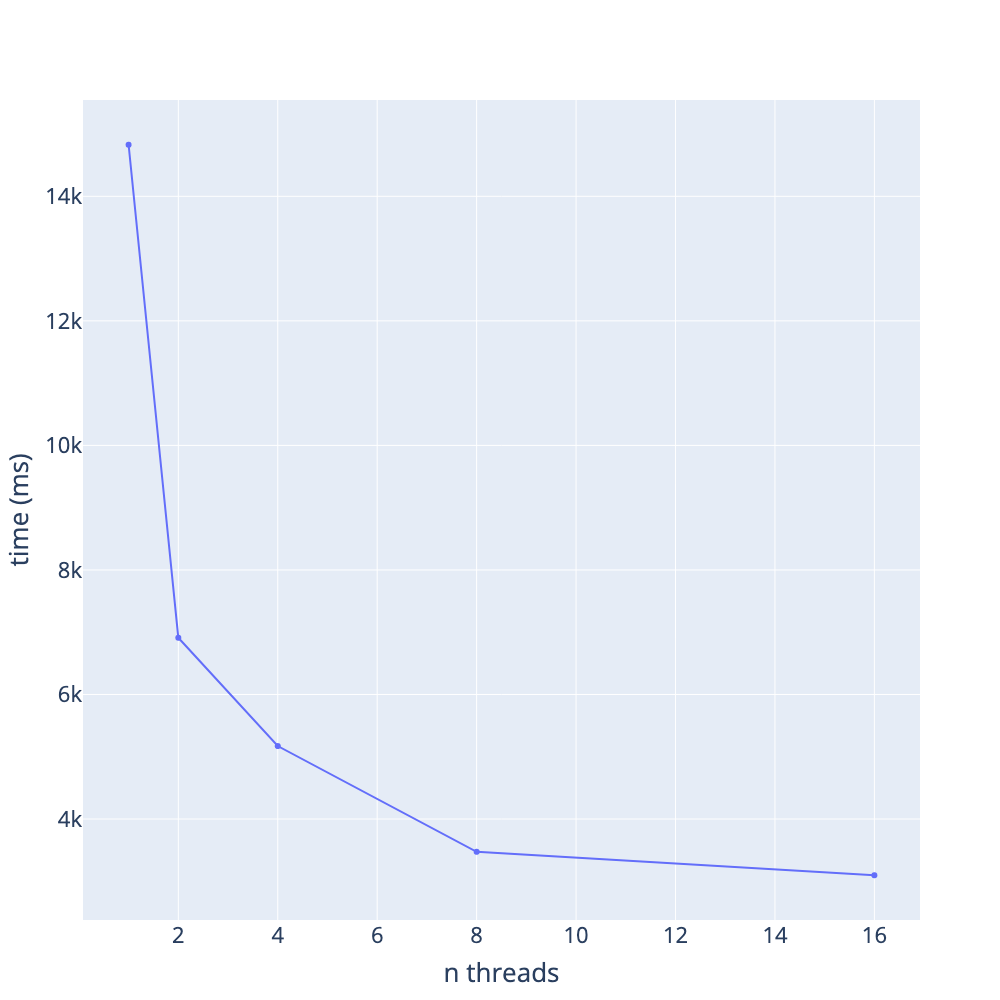
\includegraphics[width=\linewidth]{pictures/Lpi_128_time_threads.png}
  \caption{Время работы от числа нитей}
\end{subfigure}%
\end{figure}


\subsubsection{Графики для N=256}

\begin{figure}[H]
\begin{subfigure}{.33\textwidth}
  \centering
  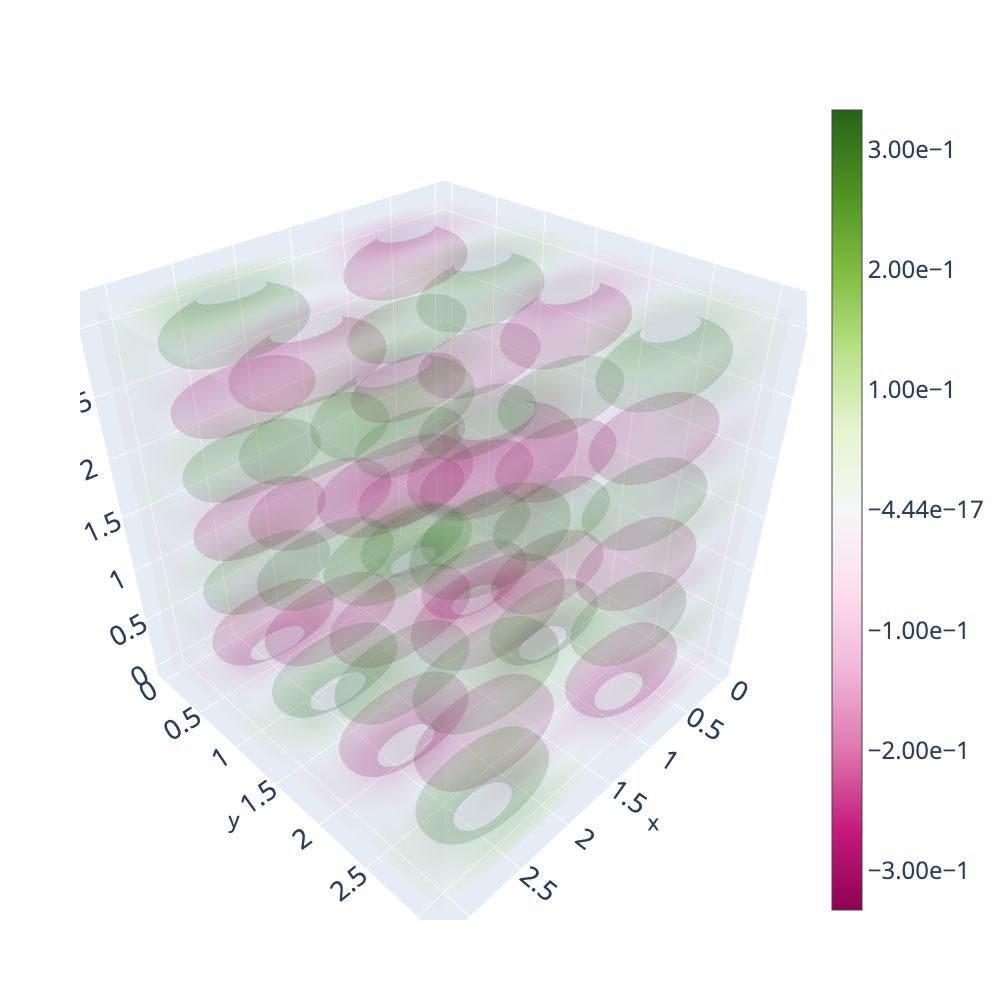
\includegraphics[width=\linewidth]{pictures/1_Lpi_256_analytical.png}
  \caption{$u_{analytical}$}
\end{subfigure}%
\begin{subfigure}{.33\textwidth}
  \centering
  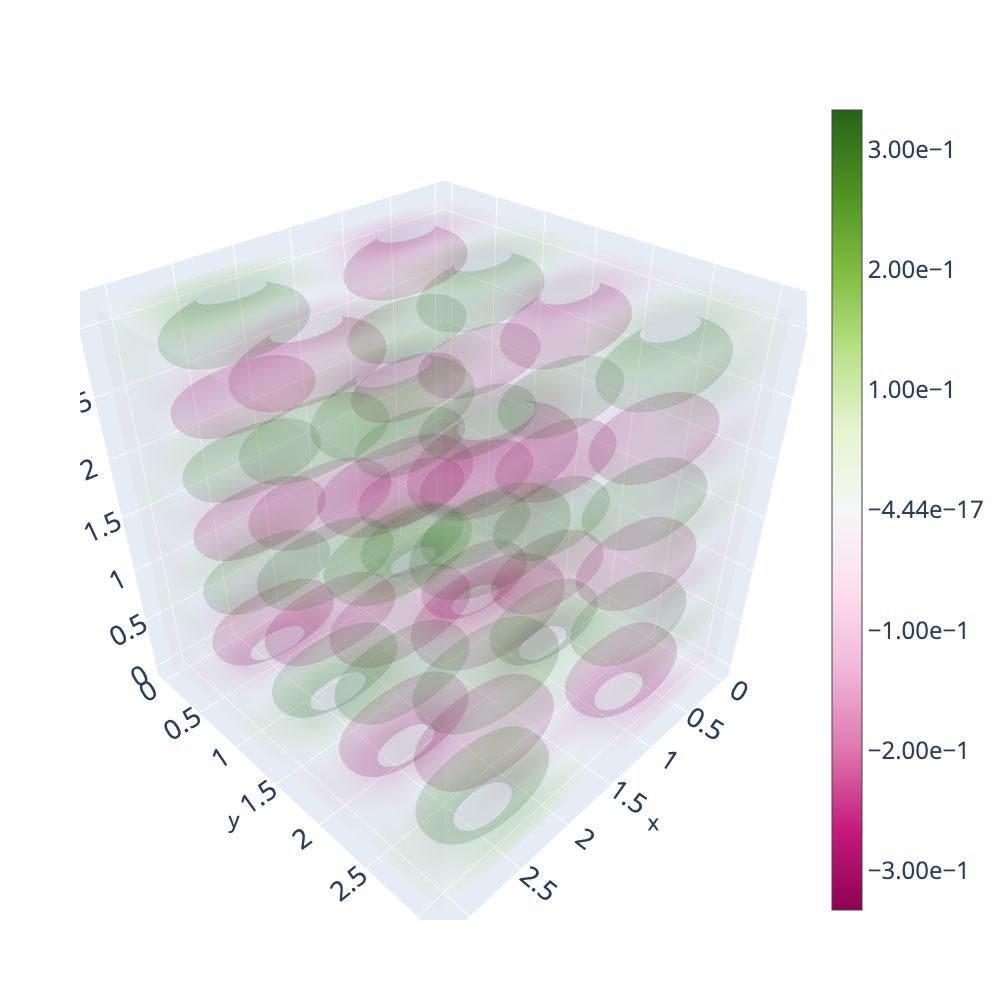
\includegraphics[width=\linewidth]{pictures/1_Lpi_256_calculated.png}
  \caption{$u_{calculated}$}
\end{subfigure}%
\begin{subfigure}{.33\textwidth}
  \centering
  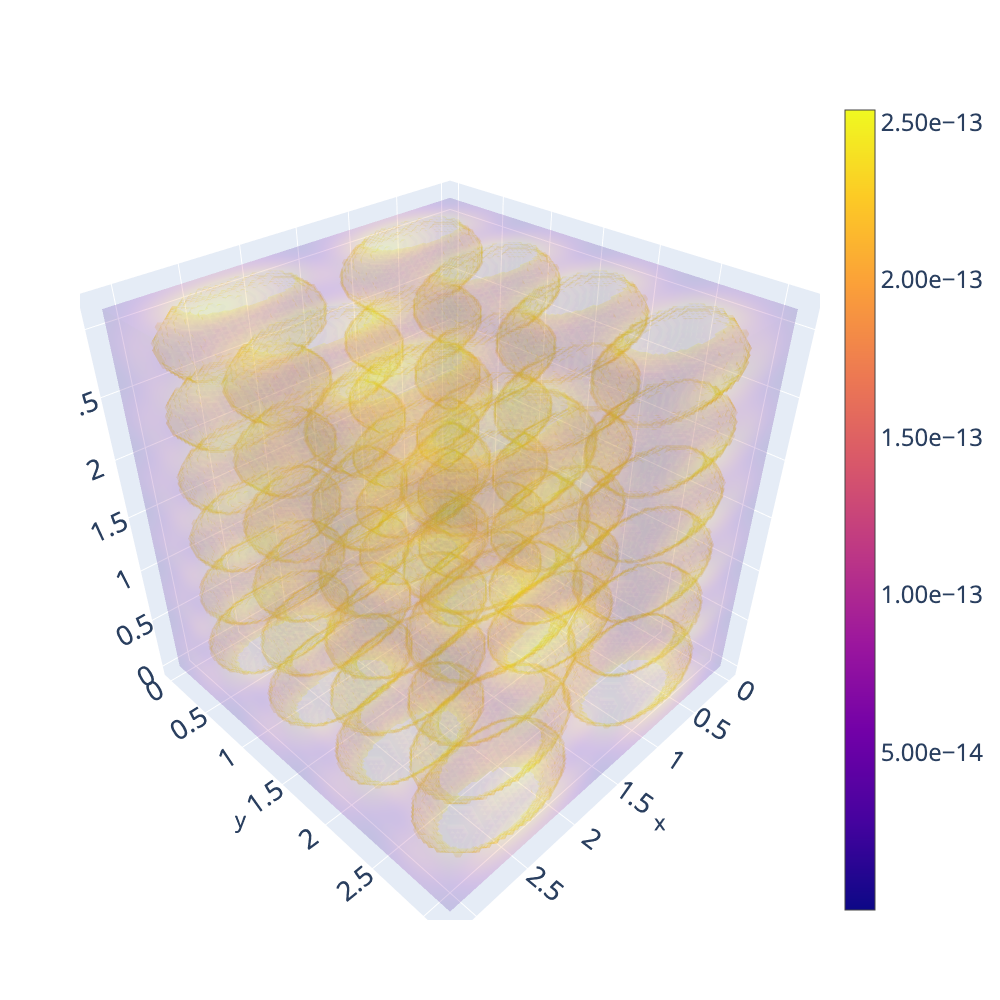
\includegraphics[width=\linewidth]{pictures/1_Lpi_256_diff.png}
  \caption{погрешность}
\end{subfigure}%
\caption{1 эпоха}
\label{fig:fig}
\end{figure}

\begin{figure}[H]
\begin{subfigure}{.33\textwidth}
  \centering
  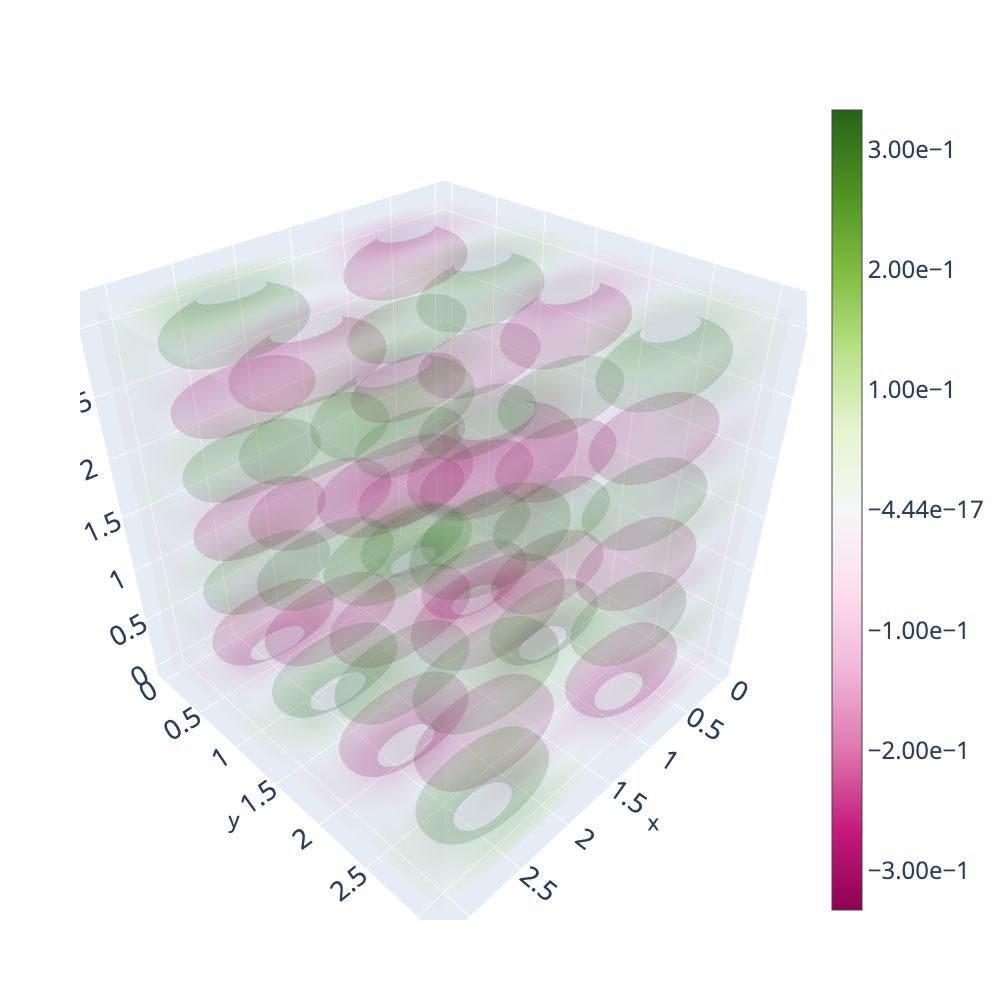
\includegraphics[width=\linewidth]{pictures/10_Lpi_256_analytical.png}
  \caption{$u_{analytical}$}
\end{subfigure}%
\begin{subfigure}{.33\textwidth}
  \centering
  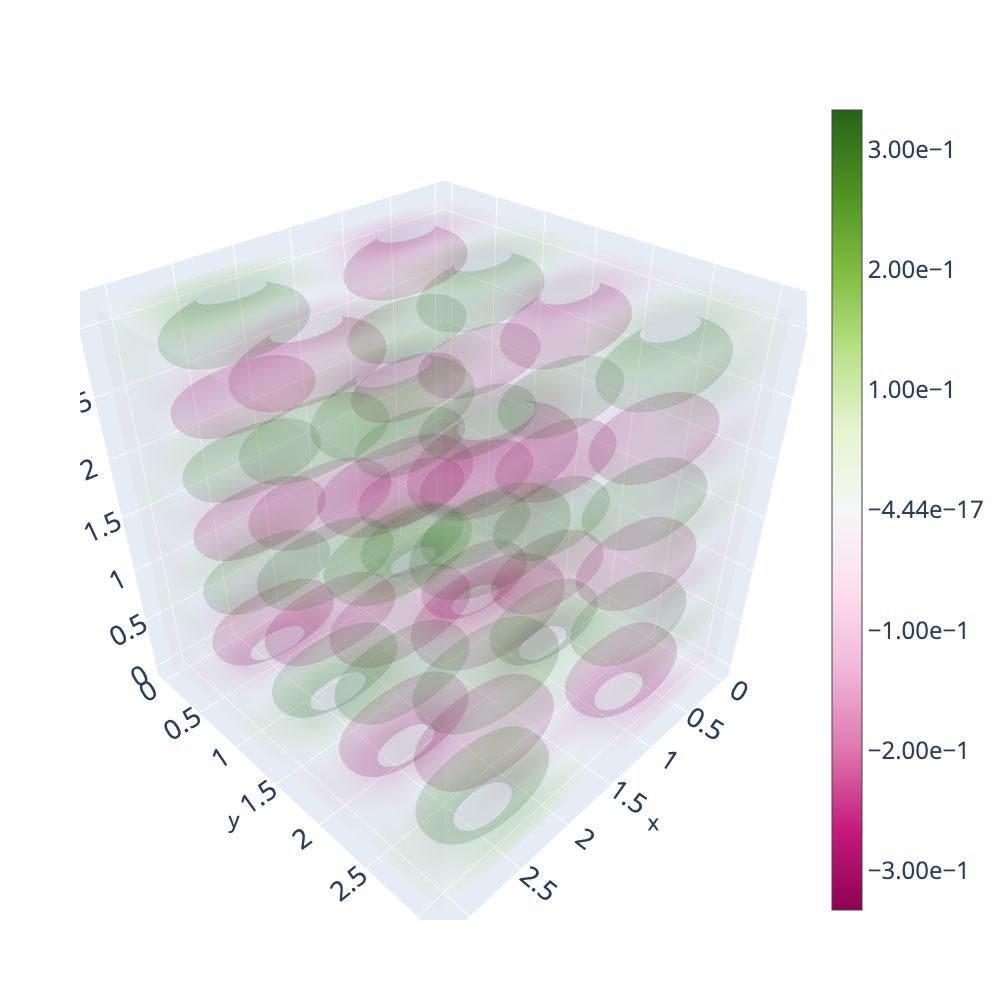
\includegraphics[width=\linewidth]{pictures/10_Lpi_256_calculated.png}
  \caption{$u_{calculated}$}
\end{subfigure}%
\begin{subfigure}{.33\textwidth}
  \centering
  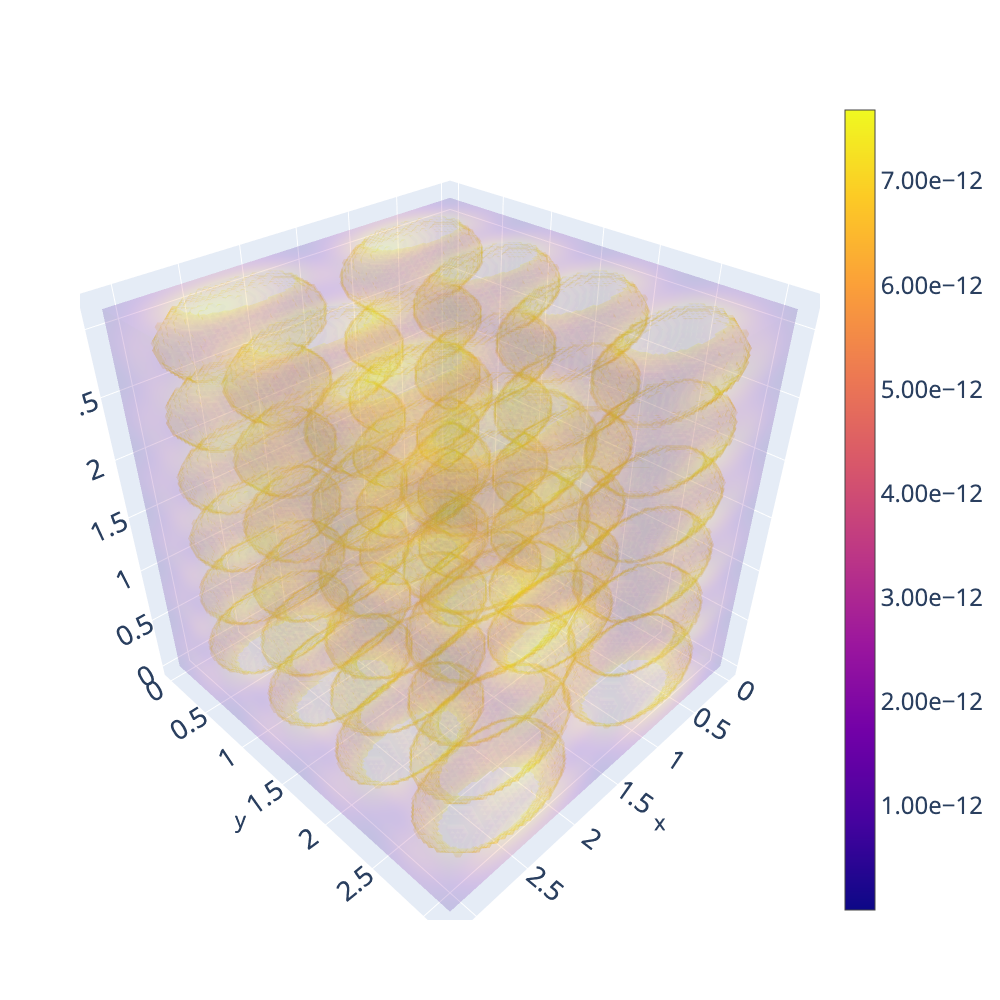
\includegraphics[width=\linewidth]{pictures/10_Lpi_256_diff.png}
  \caption{погрешность}
\end{subfigure}%
\caption{10 эпоха}
\label{fig:fig}
\end{figure}

\begin{figure}[H]
\begin{subfigure}{.33\textwidth}
  \centering
  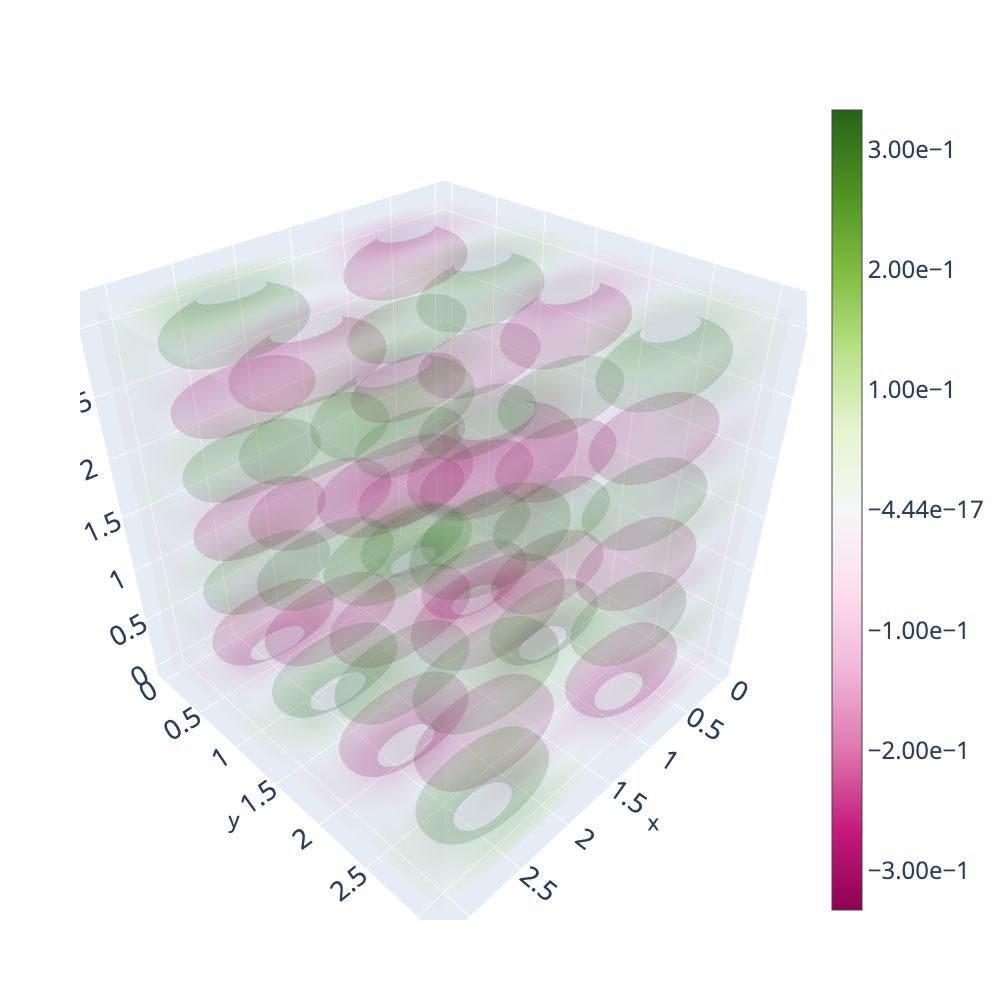
\includegraphics[width=\linewidth]{pictures/19_Lpi_256_analytical.png}
  \caption{$u_{analytical}$}
\end{subfigure}%
\begin{subfigure}{.33\textwidth}
  \centering
  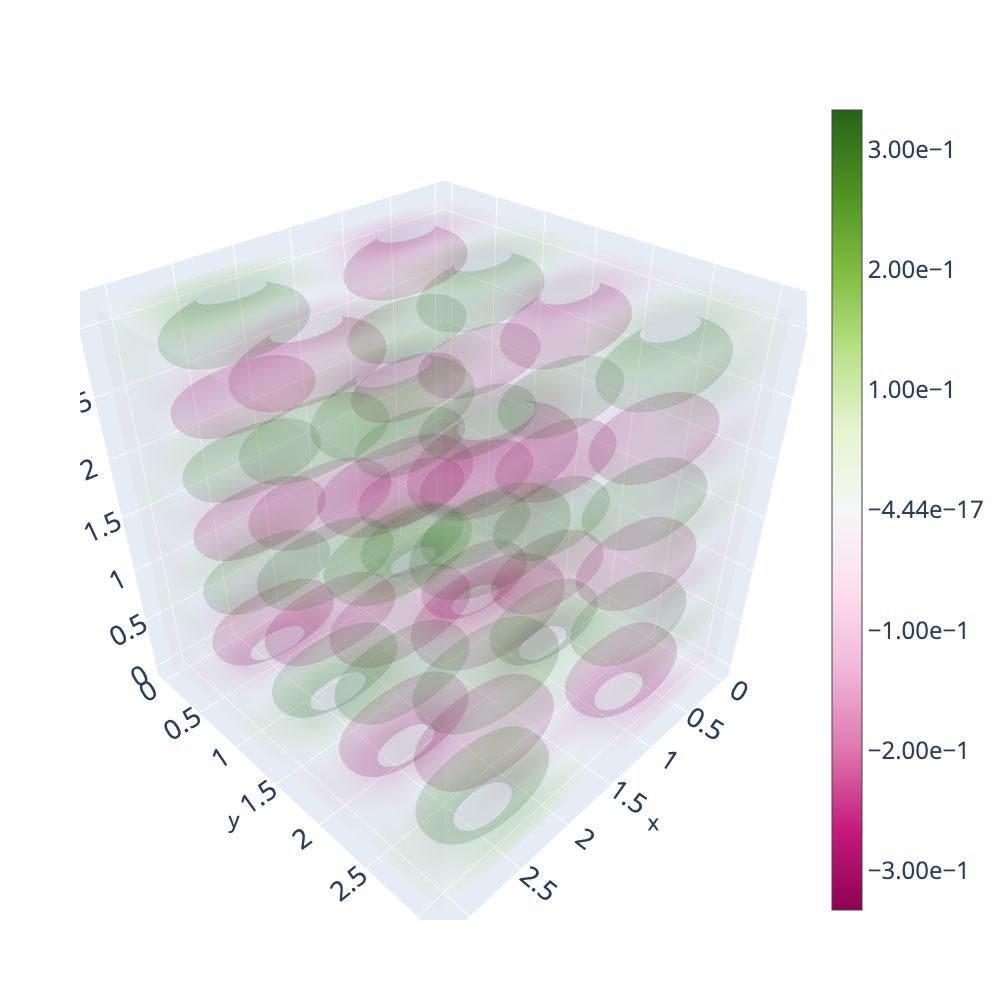
\includegraphics[width=\linewidth]{pictures/19_Lpi_256_calculated.png}
  \caption{$u_{calculated}$}
\end{subfigure}%
\begin{subfigure}{.33\textwidth}
  \centering
  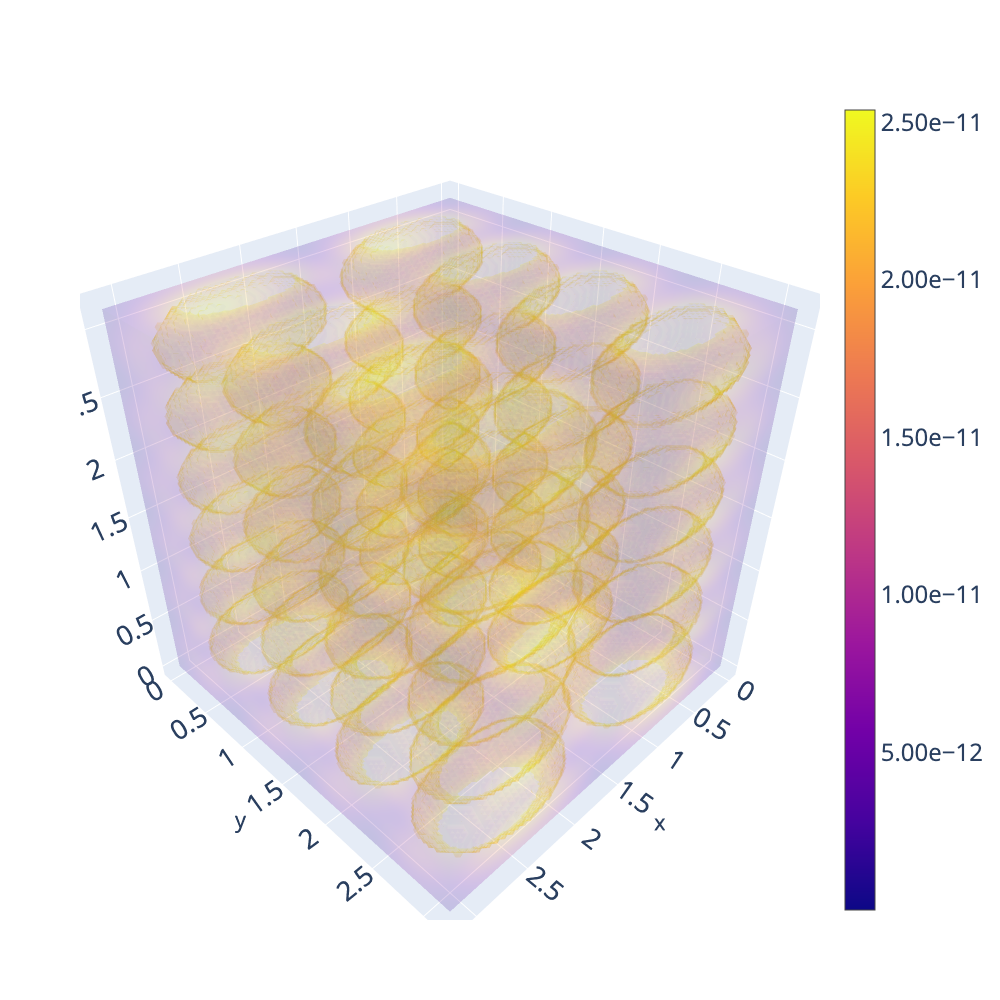
\includegraphics[width=\linewidth]{pictures/19_Lpi_256_diff.png}
  \caption{погрешность}
\end{subfigure}%
\caption{20 эпоха}
\label{fig:fig}
\end{figure}

\begin{figure}[H]
\begin{subfigure}{.5\textwidth}
  \centering
  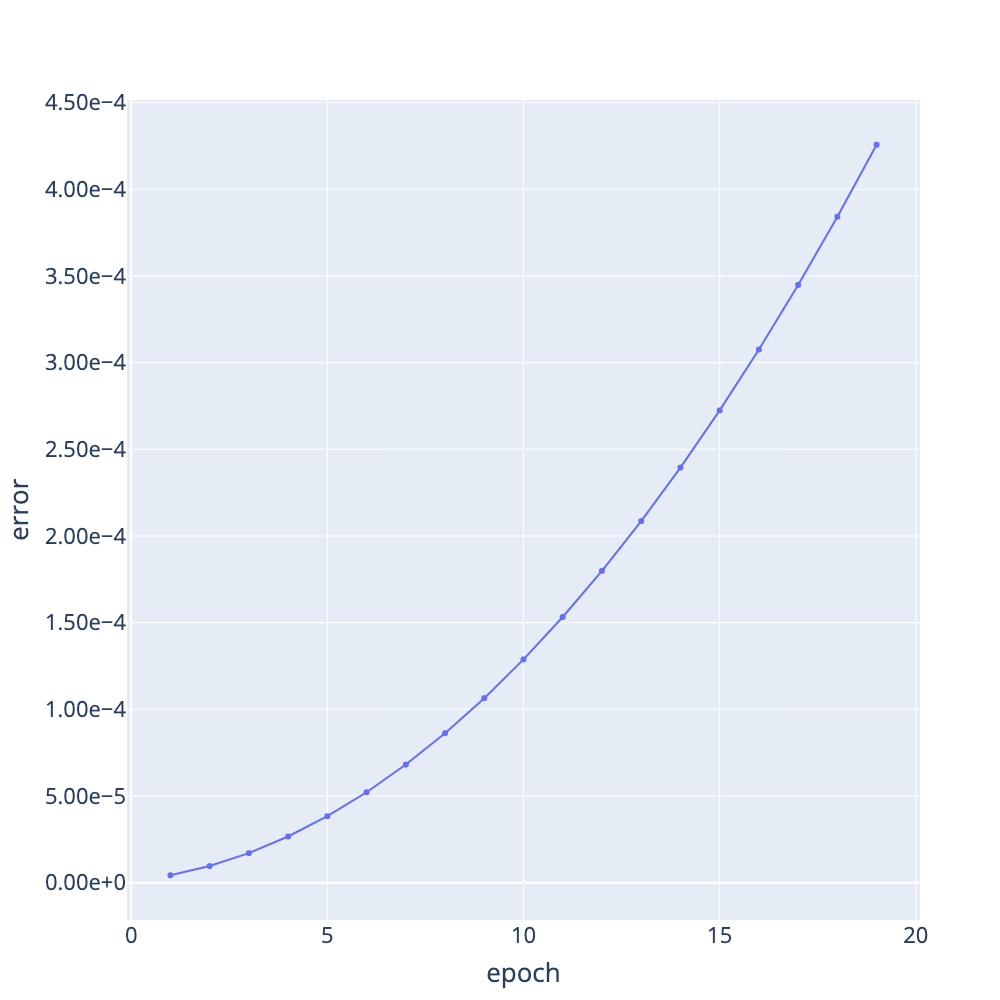
\includegraphics[width=\linewidth]{pictures/Lpi_256_err.png}
  \caption{Погрешность от эпохи}
\end{subfigure}%
\begin{subfigure}{.5\textwidth}
  \centering
  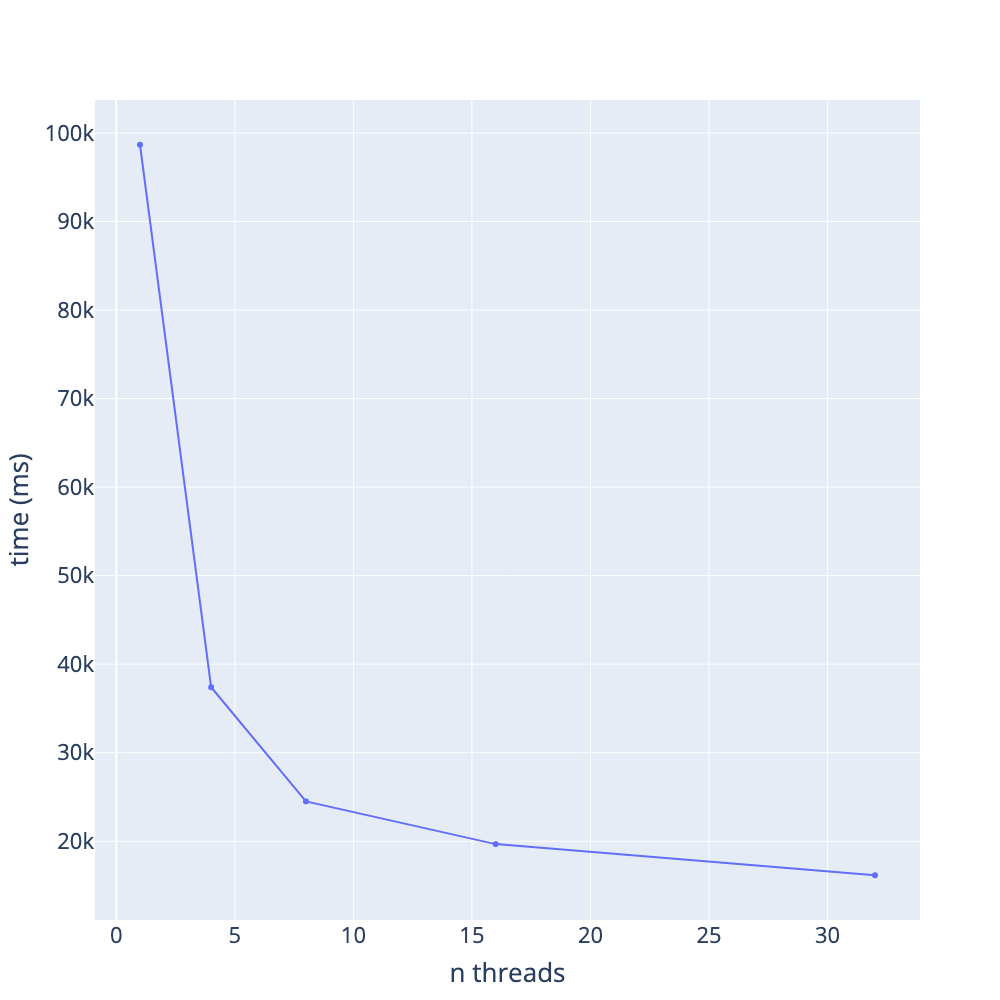
\includegraphics[width=\linewidth]{pictures/Lpi_256_time_threads.png}
  \caption{Время работы от числа нитей}
\end{subfigure}%
\end{figure}

\newpage
\section{Заключение}

На основе анализа данных о запуске программы с различным числом процессом и на различных сетках можно сделать следующие выводы:

\begin{itemize}
    \item На сетке 256 более заметно ускорение от числа нитей. Скорее всего, это связано с большей долей во времени работы программы непосредственно вычислений по сравнению с побочными задачами вроде копирования тензоров;

    \item На сетке 256 лучше видно, по какой функции расходится явная разностная схема;

    \item На сетке 256 вычисленное решение горадо ближе прилегает к аналитическому (это видно по форме поверхностей на графиках погрешности).
\end{itemize}
    

\end{document}
